\documentclass[twoside]{book}

% Packages required by doxygen
\usepackage{fixltx2e}
\usepackage{calc}
\usepackage{doxygen}
\usepackage[export]{adjustbox} % also loads graphicx
\usepackage{graphicx}
\usepackage[utf8]{inputenc}
\usepackage{makeidx}
\usepackage{multicol}
\usepackage{multirow}
\PassOptionsToPackage{warn}{textcomp}
\usepackage{textcomp}
\usepackage[nointegrals]{wasysym}
\usepackage[table]{xcolor}

% Font selection
\usepackage[T1]{fontenc}
\usepackage[scaled=.90]{helvet}
\usepackage{courier}
\usepackage{amssymb}
\usepackage{sectsty}
\renewcommand{\familydefault}{\sfdefault}
\allsectionsfont{%
  \fontseries{bc}\selectfont%
  \color{darkgray}%
}
\renewcommand{\DoxyLabelFont}{%
  \fontseries{bc}\selectfont%
  \color{darkgray}%
}
\newcommand{\+}{\discretionary{\mbox{\scriptsize$\hookleftarrow$}}{}{}}

% Page & text layout
\usepackage{geometry}
\geometry{%
  a4paper,%
  top=2.5cm,%
  bottom=2.5cm,%
  left=2.5cm,%
  right=2.5cm%
}
\tolerance=750
\hfuzz=15pt
\hbadness=750
\setlength{\emergencystretch}{15pt}
\setlength{\parindent}{0cm}
\setlength{\parskip}{3ex plus 2ex minus 2ex}
\makeatletter
\renewcommand{\paragraph}{%
  \@startsection{paragraph}{4}{0ex}{-1.0ex}{1.0ex}{%
    \normalfont\normalsize\bfseries\SS@parafont%
  }%
}
\renewcommand{\subparagraph}{%
  \@startsection{subparagraph}{5}{0ex}{-1.0ex}{1.0ex}{%
    \normalfont\normalsize\bfseries\SS@subparafont%
  }%
}
\makeatother

% Headers & footers
\usepackage{fancyhdr}
\pagestyle{fancyplain}
\fancyhead[LE]{\fancyplain{}{\bfseries\thepage}}
\fancyhead[CE]{\fancyplain{}{}}
\fancyhead[RE]{\fancyplain{}{\bfseries\leftmark}}
\fancyhead[LO]{\fancyplain{}{\bfseries\rightmark}}
\fancyhead[CO]{\fancyplain{}{}}
\fancyhead[RO]{\fancyplain{}{\bfseries\thepage}}
\fancyfoot[LE]{\fancyplain{}{}}
\fancyfoot[CE]{\fancyplain{}{}}
\fancyfoot[RE]{\fancyplain{}{\bfseries\scriptsize Generated by Doxygen }}
\fancyfoot[LO]{\fancyplain{}{\bfseries\scriptsize Generated by Doxygen }}
\fancyfoot[CO]{\fancyplain{}{}}
\fancyfoot[RO]{\fancyplain{}{}}
\renewcommand{\footrulewidth}{0.4pt}
\renewcommand{\chaptermark}[1]{%
  \markboth{#1}{}%
}
\renewcommand{\sectionmark}[1]{%
  \markright{\thesection\ #1}%
}

% Indices & bibliography
\usepackage{natbib}
\usepackage[titles]{tocloft}
\setcounter{tocdepth}{3}
\setcounter{secnumdepth}{5}
\makeindex

% Hyperlinks (required, but should be loaded last)
\usepackage{ifpdf}
\ifpdf
  \usepackage[pdftex,pagebackref=true]{hyperref}
\else
  \usepackage[ps2pdf,pagebackref=true]{hyperref}
\fi
\hypersetup{%
  colorlinks=true,%
  linkcolor=blue,%
  citecolor=blue,%
  unicode%
}

% Custom commands
\newcommand{\clearemptydoublepage}{%
  \newpage{\pagestyle{empty}\cleardoublepage}%
}

\usepackage{caption}
\captionsetup{labelsep=space,justification=centering,font={bf},singlelinecheck=off,skip=4pt,position=top}

%===== C O N T E N T S =====

\begin{document}

% Titlepage & ToC
\hypersetup{pageanchor=false,
             bookmarksnumbered=true,
             pdfencoding=unicode
            }
\pagenumbering{roman}
\begin{titlepage}
\vspace*{7cm}
\begin{center}%
{\Large Heat Conduction Equation }\\
\vspace*{1cm}
{\large Generated by Doxygen 1.8.11}\\
\end{center}
\end{titlepage}
\clearemptydoublepage
\tableofcontents
\clearemptydoublepage
\pagenumbering{arabic}
\hypersetup{pageanchor=true}

%--- Begin generated contents ---
\chapter{Hierarchical Index}
\section{Class Hierarchy}
This inheritance list is sorted roughly, but not completely, alphabetically\+:\begin{DoxyCompactList}
\item \contentsline{section}{Configuration}{\pageref{classConfiguration}}{}
\item \contentsline{section}{Job}{\pageref{classJob}}{}
\item Q\+Main\+Window\begin{DoxyCompactList}
\item \contentsline{section}{Main\+Window}{\pageref{classMainWindow}}{}
\end{DoxyCompactList}
\item \contentsline{section}{State}{\pageref{classState}}{}
\item \contentsline{section}{Statistics}{\pageref{classStatistics}}{}
\item \contentsline{section}{System}{\pageref{classSystem}}{}
\item \contentsline{section}{User}{\pageref{classUser}}{}
\item \contentsline{section}{Week}{\pageref{classWeek}}{}
\end{DoxyCompactList}

\chapter{Class Index}
\section{Class List}
Here are the classes, structs, unions and interfaces with brief descriptions\+:\begin{DoxyCompactList}
\item\contentsline{section}{\hyperlink{classConfiguration}{Configuration} \\*\hyperlink{classConfiguration}{Configuration} class }{\pageref{classConfiguration}}{}
\item\contentsline{section}{\hyperlink{classJob}{Job} \\*\hyperlink{classJob}{Job} class }{\pageref{classJob}}{}
\item\contentsline{section}{\hyperlink{classMainWindow}{Main\+Window} \\*\hyperlink{classMainWindow}{Main\+Window} class }{\pageref{classMainWindow}}{}
\item\contentsline{section}{\hyperlink{classState}{State} \\*\hyperlink{classState}{State} class }{\pageref{classState}}{}
\item\contentsline{section}{\hyperlink{classStatistics}{Statistics} \\*\hyperlink{classStatistics}{Statistics} class }{\pageref{classStatistics}}{}
\item\contentsline{section}{\hyperlink{classSystem}{System} \\*\hyperlink{classSystem}{System} class }{\pageref{classSystem}}{}
\item\contentsline{section}{\hyperlink{classUser}{User} \\*\hyperlink{classSystem}{System} class }{\pageref{classUser}}{}
\item\contentsline{section}{\hyperlink{classWeek}{Week} \\*\hyperlink{classWeek}{Week} class }{\pageref{classWeek}}{}
\end{DoxyCompactList}

\chapter{Class Documentation}
\hypertarget{classConfiguration}{}\section{Configuration Class Reference}
\label{classConfiguration}\index{Configuration@{Configuration}}


\hyperlink{classConfiguration}{Configuration} class.  




{\ttfamily \#include $<$configuration.\+h$>$}

\subsection*{Public Member Functions}
\begin{DoxyCompactItemize}
\item 
\hyperlink{classConfiguration_a779947337bf652f0e773cb29f37f14ba}{Configuration} ()
\begin{DoxyCompactList}\small\item\em \hyperlink{classConfiguration}{Configuration} object default contructor. \end{DoxyCompactList}\item 
unsigned int \hyperlink{classConfiguration_ace5f9aa5555419110b7df4e6eb664931}{get\+\_\+users\+\_\+nr} ()
\begin{DoxyCompactList}\small\item\em Public method. Returns the number of users when this value is not generated randomly. \end{DoxyCompactList}\item 
unsigned int \hyperlink{classConfiguration_a09999edf2be5ece81d64ea825c7fd339}{get\+\_\+users\+\_\+nr\+\_\+min} ()
\begin{DoxyCompactList}\small\item\em Public method. Returns the lower limit of randomly generated values of number of users. \end{DoxyCompactList}\item 
unsigned int \hyperlink{classConfiguration_a2ce1f2af9f9733712a8cbbfb7f5b277c}{get\+\_\+users\+\_\+nr\+\_\+max} ()
\begin{DoxyCompactList}\small\item\em Public method. Returns the upper limit of randomly generated values of number of users. \end{DoxyCompactList}\item 
bool \hyperlink{classConfiguration_a3c6d60da873c53d2a785e64f67668c4f}{is\+\_\+users\+\_\+nr\+\_\+random} ()
\begin{DoxyCompactList}\small\item\em Public method. Returns true if the number of users is generated randomly, and false if it\textquotesingle{}s not. \end{DoxyCompactList}\item 
unsigned int \hyperlink{classConfiguration_a09d80d794d6614c7bcbdf12b49835f02}{get\+\_\+jobs\+\_\+nr} ()
\begin{DoxyCompactList}\small\item\em Public method. Returns the number of jobs when this value is not generated randomly. \end{DoxyCompactList}\item 
unsigned int \hyperlink{classConfiguration_a3d224269091e27f9595485ec5d4b0467}{get\+\_\+jobs\+\_\+nr\+\_\+min} ()
\begin{DoxyCompactList}\small\item\em Public method. Returns the lower limit of randomly generated values of number of jobs. \end{DoxyCompactList}\item 
unsigned int \hyperlink{classConfiguration_a19e2080f751736cf98017f6e40533629}{get\+\_\+jobs\+\_\+nr\+\_\+max} ()
\begin{DoxyCompactList}\small\item\em Public method. Returns the upper limit of randomly generated values of number of jobs. \end{DoxyCompactList}\item 
bool \hyperlink{classConfiguration_ae35b4429de406ed81c1be1ae54bfc3d7}{is\+\_\+jobs\+\_\+nr\+\_\+random} ()
\begin{DoxyCompactList}\small\item\em Public method. Returns true if the number of jobs is generated randomly, and false if it\textquotesingle{}s not. \end{DoxyCompactList}\item 
unsigned int \hyperlink{classConfiguration_a3255f4b61deb08b21a39251b9dc4d2b4}{get\+\_\+cores\+\_\+nr} ()
\begin{DoxyCompactList}\small\item\em Public method. Returns the number of cores per node. \end{DoxyCompactList}\item 
unsigned int \hyperlink{classConfiguration_aafbd7647fdc9447cf882083a0be02263}{get\+\_\+nodes\+\_\+nr} ()
\begin{DoxyCompactList}\small\item\em Public method. Returns the total number of system nodes. \end{DoxyCompactList}\item 
double \hyperlink{classConfiguration_a65edb47ed369c917d275812bba3e46c8}{get\+\_\+usage\+\_\+price} ()
\begin{DoxyCompactList}\small\item\em Public method. Returns the usage price of the system per core second. \end{DoxyCompactList}\item 
double \hyperlink{classConfiguration_a3a3d1dd3bb8ef78b09fbed9954ec1c8f}{get\+\_\+operational\+\_\+cost} ()
\begin{DoxyCompactList}\small\item\em Public method. Returns the operational cost of the system per second. \end{DoxyCompactList}\item 
double \hyperlink{classConfiguration_af7b5ce431f51f8848e32ba76af63c531}{get\+\_\+student\+\_\+budget} ()
\begin{DoxyCompactList}\small\item\em Public method. Returns the student budget. \end{DoxyCompactList}\item 
double \hyperlink{classConfiguration_a3a6291edf176db0bdcc4b88c529a6447}{get\+\_\+student\+\_\+budget\+\_\+min} ()
\begin{DoxyCompactList}\small\item\em Public method. Returns the lower limit of randomly generated values of student budget. \end{DoxyCompactList}\item 
double \hyperlink{classConfiguration_a9b8da18d74cdedc6d779c560d714fbc1}{get\+\_\+student\+\_\+budget\+\_\+max} ()
\begin{DoxyCompactList}\small\item\em Public method. Returns the upper limit of randomly generated values of student budget. \end{DoxyCompactList}\item 
bool \hyperlink{classConfiguration_ac5422f301431649bfc63319bf4b0b2e9}{is\+\_\+student\+\_\+budget\+\_\+random} ()
\begin{DoxyCompactList}\small\item\em Public method. Returns true if the student budget is generated randomly, and false if it\textquotesingle{}s not. \end{DoxyCompactList}\item 
double \hyperlink{classConfiguration_a9555ca72e72aacb78585365a328c3c9f}{get\+\_\+researcher\+\_\+budget} ()
\begin{DoxyCompactList}\small\item\em Public method. Returns the researcher budget. \end{DoxyCompactList}\item 
double \hyperlink{classConfiguration_aefb667cc98649f5a32fc16665c6b28c9}{get\+\_\+researcher\+\_\+budget\+\_\+min} ()
\begin{DoxyCompactList}\small\item\em Public method. Returns the lower limit of randomly generated values of researcher budget. \end{DoxyCompactList}\item 
double \hyperlink{classConfiguration_ac4ae307e11f10c5cf1a0e32d14621948}{get\+\_\+researcher\+\_\+budget\+\_\+max} ()
\begin{DoxyCompactList}\small\item\em Public method. Returns the upper limit of randomly generated values of researcher budget. \end{DoxyCompactList}\item 
bool \hyperlink{classConfiguration_aaf2bcbe58e2a4844c2f6d74a94191ac5}{is\+\_\+researcher\+\_\+budget\+\_\+random} ()
\begin{DoxyCompactList}\small\item\em Public method. Returns true if the researcher budget is generated randomly, and false if it\textquotesingle{}s not. \end{DoxyCompactList}\item 
time\+\_\+t \hyperlink{classConfiguration_aeb49a69a8a52a9603d5e46180a73b770}{get\+\_\+time} ()
\begin{DoxyCompactList}\small\item\em Public method. Returns the starting time of the simulation in U\+N\+IX timestamp format. \end{DoxyCompactList}\item 
unsigned long long int \hyperlink{classConfiguration_a4f94d71b89f3fdea573050da6fe5e0e6}{get\+\_\+requests\+\_\+span} ()
\begin{DoxyCompactList}\small\item\em Public method. Returns the requests time span in seconds. \end{DoxyCompactList}\item 
void \hyperlink{classConfiguration_a057a8d808d077731c582ec280a897bf9}{set\+\_\+student\+\_\+random} (bool random)
\begin{DoxyCompactList}\small\item\em Public method. Changes the way the student budget is defined. \end{DoxyCompactList}\item 
void \hyperlink{classConfiguration_a6230496122b25f645092fe3b9896f883}{set\+\_\+researcher\+\_\+random} (bool random)
\begin{DoxyCompactList}\small\item\em Public method. Changes the way the researcher budget is defined. \end{DoxyCompactList}\item 
void \hyperlink{classConfiguration_aedf812b154b8cc8b3db322f6d969ca59}{set\+\_\+users\+\_\+random} (bool random)
\begin{DoxyCompactList}\small\item\em Public method. Changes the way the number of users is defined. \end{DoxyCompactList}\item 
void \hyperlink{classConfiguration_acd24051b1759e61132d6653e0df9dfe4}{set\+\_\+jobs\+\_\+random} (bool random)
\begin{DoxyCompactList}\small\item\em Public method. Changes the way the number of jobs is defined. \end{DoxyCompactList}\item 
void \hyperlink{classConfiguration_a1d5547d2f203074882e1d6d3c5ddbb8a}{set\+\_\+now} (bool now)
\begin{DoxyCompactList}\small\item\em Public method. Changes whether the simulation starting time is the present date or not. \end{DoxyCompactList}\item 
void \hyperlink{classConfiguration_a7d9e089372333b0c1ec93c7fdbd297f2}{set\+\_\+time} (time\+\_\+t time)
\begin{DoxyCompactList}\small\item\em Public method. Defines a date value for non-\/present starting dates simulations. \end{DoxyCompactList}\item 
void \hyperlink{classConfiguration_a0b9459ad48edbac60dcd8962910653a2}{set\+\_\+usage\+\_\+price} (double usage\+\_\+price)
\begin{DoxyCompactList}\small\item\em Public method. Defines the usage price of the system per core second. \end{DoxyCompactList}\item 
void \hyperlink{classConfiguration_a31284f3adcd959a1092a27efb5742452}{set\+\_\+operational\+\_\+cost} (double operational\+\_\+cost)
\begin{DoxyCompactList}\small\item\em Public method. Defines the operational cost of the system per core second. \end{DoxyCompactList}\item 
void \hyperlink{classConfiguration_ac74a221224fbf7db75c3afa47fba2d61}{set\+\_\+nodes\+\_\+nr} (unsigned int nodes\+\_\+nr)
\begin{DoxyCompactList}\small\item\em Public method. Defines the total number of system nodes. \end{DoxyCompactList}\item 
void \hyperlink{classConfiguration_a299244e0d054564921a3344b14e94973}{set\+\_\+cores\+\_\+nr} (unsigned int cores\+\_\+nr)
\begin{DoxyCompactList}\small\item\em Public method. Defines the number of cores per node. \end{DoxyCompactList}\item 
void \hyperlink{classConfiguration_a00fb5adcb5145810133ef68a662dca91}{set\+\_\+student\+\_\+budget} (double budget)
\begin{DoxyCompactList}\small\item\em Public method. Defines the student budget of a new simulation. \end{DoxyCompactList}\item 
void \hyperlink{classConfiguration_ae6cc1bfec9271811e94df8a6bba264f0}{set\+\_\+student\+\_\+budget\+\_\+min} (double min)
\begin{DoxyCompactList}\small\item\em Public method. Defines the lower limit student budgets when this value is randomly generated. \end{DoxyCompactList}\item 
void \hyperlink{classConfiguration_aba1e5f9fe84879c3628382096015cd94}{set\+\_\+student\+\_\+budget\+\_\+max} (double max)
\begin{DoxyCompactList}\small\item\em Public method. Defines the upper limit student budgets when this value is randomly generated. \end{DoxyCompactList}\item 
void \hyperlink{classConfiguration_a92a48764d5717464989aed435de76bc6}{set\+\_\+researcher\+\_\+budget} (double budget)
\begin{DoxyCompactList}\small\item\em Public method. Defines the researcher budget of a new simulation. \end{DoxyCompactList}\item 
void \hyperlink{classConfiguration_a8fb6a2c896ca9a98ffa605b84b6ddde7}{set\+\_\+researcher\+\_\+budget\+\_\+min} (double min)
\begin{DoxyCompactList}\small\item\em Public method. Defines the lower limit researcher budgets when this value is randomly generated. \end{DoxyCompactList}\item 
void \hyperlink{classConfiguration_add79fec297e6e38097b3a0b9968c8d2c}{set\+\_\+researcher\+\_\+budget\+\_\+max} (double max)
\begin{DoxyCompactList}\small\item\em Public method. Defines the upper limit researcher budgets when this value is randomly generated. \end{DoxyCompactList}\item 
void \hyperlink{classConfiguration_a915a2e408d2c2b95e0e7cfe4a5842c2d}{set\+\_\+jobs\+\_\+nr} (unsigned int nr)
\begin{DoxyCompactList}\small\item\em Public method. Defines the number of jobs of a new simulation. \end{DoxyCompactList}\item 
void \hyperlink{classConfiguration_a5132f41c23a73bb4fded422f325cbbe6}{set\+\_\+jobs\+\_\+nr\+\_\+min} (unsigned int min)
\begin{DoxyCompactList}\small\item\em Public method. Defines the lower limit of jobs when this value is randomly generated. \end{DoxyCompactList}\item 
void \hyperlink{classConfiguration_a288259d1e0c47f99ddd0feec5ade6d93}{set\+\_\+jobs\+\_\+nr\+\_\+max} (unsigned int max)
\begin{DoxyCompactList}\small\item\em Public method. Defines the upper limit of jobs when this value is randomly generated. \end{DoxyCompactList}\item 
void \hyperlink{classConfiguration_a0e27b300afd52eb1a07f202ee8a05746}{set\+\_\+users\+\_\+nr} (unsigned int nr)
\begin{DoxyCompactList}\small\item\em Public method. Defines the number of users of a new simulation. \end{DoxyCompactList}\item 
void \hyperlink{classConfiguration_aca5c8d3046cc871ce78b0c6ef0d3cda6}{set\+\_\+users\+\_\+nr\+\_\+min} (unsigned int min)
\begin{DoxyCompactList}\small\item\em Public method. Defines the lower limit of users when this value is randomly generated. \end{DoxyCompactList}\item 
void \hyperlink{classConfiguration_af5b4e0360ab5bc2d5535e993850e2f23}{set\+\_\+users\+\_\+nr\+\_\+max} (unsigned int max)
\begin{DoxyCompactList}\small\item\em Public method. Defines the upper limit of users when this value is randomly generated. \end{DoxyCompactList}\item 
void \hyperlink{classConfiguration_a485b378ed96796fd7a7ca17ace180060}{set\+\_\+requests\+\_\+span} (unsigned long long int span)
\begin{DoxyCompactList}\small\item\em Public method. Defines the requests time span. \end{DoxyCompactList}\end{DoxyCompactItemize}


\subsection{Detailed Description}
\hyperlink{classConfiguration}{Configuration} class. 

This object includes the input values of the simulation. 

\subsection{Constructor \& Destructor Documentation}
\index{Configuration@{Configuration}!Configuration@{Configuration}}
\index{Configuration@{Configuration}!Configuration@{Configuration}}
\subsubsection[{\texorpdfstring{Configuration()}{Configuration()}}]{\setlength{\rightskip}{0pt plus 5cm}Configuration\+::\+Configuration (
\begin{DoxyParamCaption}
{}
\end{DoxyParamCaption}
)}\hypertarget{classConfiguration_a779947337bf652f0e773cb29f37f14ba}{}\label{classConfiguration_a779947337bf652f0e773cb29f37f14ba}


\hyperlink{classConfiguration}{Configuration} object default contructor. 

Private time\+\_\+t. Start time of the simulation.

Initializes a \hyperlink{classConfiguration}{Configuration} object.

Default contructor of configuration. The default input values are defined in the \char`\"{}utils.\+h\char`\"{} header file. 

\subsection{Member Function Documentation}
\index{Configuration@{Configuration}!get\+\_\+cores\+\_\+nr@{get\+\_\+cores\+\_\+nr}}
\index{get\+\_\+cores\+\_\+nr@{get\+\_\+cores\+\_\+nr}!Configuration@{Configuration}}
\subsubsection[{\texorpdfstring{get\+\_\+cores\+\_\+nr()}{get_cores_nr()}}]{\setlength{\rightskip}{0pt plus 5cm}unsigned int Configuration\+::get\+\_\+cores\+\_\+nr (
\begin{DoxyParamCaption}
{}
\end{DoxyParamCaption}
)}\hypertarget{classConfiguration_a3255f4b61deb08b21a39251b9dc4d2b4}{}\label{classConfiguration_a3255f4b61deb08b21a39251b9dc4d2b4}


Public method. Returns the number of cores per node. 

\begin{DoxyReturn}{Returns}
unsigned int. The number of cores per node.
\end{DoxyReturn}
Ŕeturns the number of cores per node. \index{Configuration@{Configuration}!get\+\_\+jobs\+\_\+nr@{get\+\_\+jobs\+\_\+nr}}
\index{get\+\_\+jobs\+\_\+nr@{get\+\_\+jobs\+\_\+nr}!Configuration@{Configuration}}
\subsubsection[{\texorpdfstring{get\+\_\+jobs\+\_\+nr()}{get_jobs_nr()}}]{\setlength{\rightskip}{0pt plus 5cm}unsigned int Configuration\+::get\+\_\+jobs\+\_\+nr (
\begin{DoxyParamCaption}
{}
\end{DoxyParamCaption}
)}\hypertarget{classConfiguration_a09d80d794d6614c7bcbdf12b49835f02}{}\label{classConfiguration_a09d80d794d6614c7bcbdf12b49835f02}


Public method. Returns the number of jobs when this value is not generated randomly. 

\begin{DoxyReturn}{Returns}
unsigned int. The number of jobs.
\end{DoxyReturn}
Ŕeturns a constant value if the variable \char`\"{}jobs\+\_\+random\char`\"{} is false, and a random value between two established limits if not. \index{Configuration@{Configuration}!get\+\_\+jobs\+\_\+nr\+\_\+max@{get\+\_\+jobs\+\_\+nr\+\_\+max}}
\index{get\+\_\+jobs\+\_\+nr\+\_\+max@{get\+\_\+jobs\+\_\+nr\+\_\+max}!Configuration@{Configuration}}
\subsubsection[{\texorpdfstring{get\+\_\+jobs\+\_\+nr\+\_\+max()}{get_jobs_nr_max()}}]{\setlength{\rightskip}{0pt plus 5cm}unsigned int Configuration\+::get\+\_\+jobs\+\_\+nr\+\_\+max (
\begin{DoxyParamCaption}
{}
\end{DoxyParamCaption}
)}\hypertarget{classConfiguration_a19e2080f751736cf98017f6e40533629}{}\label{classConfiguration_a19e2080f751736cf98017f6e40533629}


Public method. Returns the upper limit of randomly generated values of number of jobs. 

\begin{DoxyReturn}{Returns}
unsigned int. The upper limit.
\end{DoxyReturn}
Ŕeturns the upper limit of randomly generated values of jobs numbers. \index{Configuration@{Configuration}!get\+\_\+jobs\+\_\+nr\+\_\+min@{get\+\_\+jobs\+\_\+nr\+\_\+min}}
\index{get\+\_\+jobs\+\_\+nr\+\_\+min@{get\+\_\+jobs\+\_\+nr\+\_\+min}!Configuration@{Configuration}}
\subsubsection[{\texorpdfstring{get\+\_\+jobs\+\_\+nr\+\_\+min()}{get_jobs_nr_min()}}]{\setlength{\rightskip}{0pt plus 5cm}unsigned int Configuration\+::get\+\_\+jobs\+\_\+nr\+\_\+min (
\begin{DoxyParamCaption}
{}
\end{DoxyParamCaption}
)}\hypertarget{classConfiguration_a3d224269091e27f9595485ec5d4b0467}{}\label{classConfiguration_a3d224269091e27f9595485ec5d4b0467}


Public method. Returns the lower limit of randomly generated values of number of jobs. 

\begin{DoxyReturn}{Returns}
unsigned int. The lower limit.
\end{DoxyReturn}
Ŕeturns the lower limit of randomly generated values of jobs numbers. \index{Configuration@{Configuration}!get\+\_\+nodes\+\_\+nr@{get\+\_\+nodes\+\_\+nr}}
\index{get\+\_\+nodes\+\_\+nr@{get\+\_\+nodes\+\_\+nr}!Configuration@{Configuration}}
\subsubsection[{\texorpdfstring{get\+\_\+nodes\+\_\+nr()}{get_nodes_nr()}}]{\setlength{\rightskip}{0pt plus 5cm}unsigned int Configuration\+::get\+\_\+nodes\+\_\+nr (
\begin{DoxyParamCaption}
{}
\end{DoxyParamCaption}
)}\hypertarget{classConfiguration_aafbd7647fdc9447cf882083a0be02263}{}\label{classConfiguration_aafbd7647fdc9447cf882083a0be02263}


Public method. Returns the total number of system nodes. 

\begin{DoxyReturn}{Returns}
unsigned int. The number of nodes.
\end{DoxyReturn}
Ŕeturns the total number of nodes. \index{Configuration@{Configuration}!get\+\_\+operational\+\_\+cost@{get\+\_\+operational\+\_\+cost}}
\index{get\+\_\+operational\+\_\+cost@{get\+\_\+operational\+\_\+cost}!Configuration@{Configuration}}
\subsubsection[{\texorpdfstring{get\+\_\+operational\+\_\+cost()}{get_operational_cost()}}]{\setlength{\rightskip}{0pt plus 5cm}double Configuration\+::get\+\_\+operational\+\_\+cost (
\begin{DoxyParamCaption}
{}
\end{DoxyParamCaption}
)}\hypertarget{classConfiguration_a3a3d1dd3bb8ef78b09fbed9954ec1c8f}{}\label{classConfiguration_a3a3d1dd3bb8ef78b09fbed9954ec1c8f}


Public method. Returns the operational cost of the system per second. 

\begin{DoxyReturn}{Returns}
double. Operational cost of the system per second.
\end{DoxyReturn}
Ŕeturns the operational cost of the system per second. \index{Configuration@{Configuration}!get\+\_\+requests\+\_\+span@{get\+\_\+requests\+\_\+span}}
\index{get\+\_\+requests\+\_\+span@{get\+\_\+requests\+\_\+span}!Configuration@{Configuration}}
\subsubsection[{\texorpdfstring{get\+\_\+requests\+\_\+span()}{get_requests_span()}}]{\setlength{\rightskip}{0pt plus 5cm}unsigned long long int Configuration\+::get\+\_\+requests\+\_\+span (
\begin{DoxyParamCaption}
{}
\end{DoxyParamCaption}
)}\hypertarget{classConfiguration_a4f94d71b89f3fdea573050da6fe5e0e6}{}\label{classConfiguration_a4f94d71b89f3fdea573050da6fe5e0e6}


Public method. Returns the requests time span in seconds. 

\begin{DoxyReturn}{Returns}
time\+\_\+t. Requests time span.
\end{DoxyReturn}
Ŕeturns the requests time span in seconds. \index{Configuration@{Configuration}!get\+\_\+researcher\+\_\+budget@{get\+\_\+researcher\+\_\+budget}}
\index{get\+\_\+researcher\+\_\+budget@{get\+\_\+researcher\+\_\+budget}!Configuration@{Configuration}}
\subsubsection[{\texorpdfstring{get\+\_\+researcher\+\_\+budget()}{get_researcher_budget()}}]{\setlength{\rightskip}{0pt plus 5cm}double Configuration\+::get\+\_\+researcher\+\_\+budget (
\begin{DoxyParamCaption}
{}
\end{DoxyParamCaption}
)}\hypertarget{classConfiguration_a9555ca72e72aacb78585365a328c3c9f}{}\label{classConfiguration_a9555ca72e72aacb78585365a328c3c9f}


Public method. Returns the researcher budget. 

\begin{DoxyReturn}{Returns}
double. Student budget value.
\end{DoxyReturn}
Ŕeturns a constant value if the variable \char`\"{}student\+\_\+random\char`\"{} is false, and a random value between two established limits if not. \index{Configuration@{Configuration}!get\+\_\+researcher\+\_\+budget\+\_\+max@{get\+\_\+researcher\+\_\+budget\+\_\+max}}
\index{get\+\_\+researcher\+\_\+budget\+\_\+max@{get\+\_\+researcher\+\_\+budget\+\_\+max}!Configuration@{Configuration}}
\subsubsection[{\texorpdfstring{get\+\_\+researcher\+\_\+budget\+\_\+max()}{get_researcher_budget_max()}}]{\setlength{\rightskip}{0pt plus 5cm}double Configuration\+::get\+\_\+researcher\+\_\+budget\+\_\+max (
\begin{DoxyParamCaption}
{}
\end{DoxyParamCaption}
)}\hypertarget{classConfiguration_ac4ae307e11f10c5cf1a0e32d14621948}{}\label{classConfiguration_ac4ae307e11f10c5cf1a0e32d14621948}


Public method. Returns the upper limit of randomly generated values of researcher budget. 

\begin{DoxyReturn}{Returns}
double. The upper limit of researcher budget.
\end{DoxyReturn}
Ŕeturns the upper limit of a randomly generated researcher budget. \index{Configuration@{Configuration}!get\+\_\+researcher\+\_\+budget\+\_\+min@{get\+\_\+researcher\+\_\+budget\+\_\+min}}
\index{get\+\_\+researcher\+\_\+budget\+\_\+min@{get\+\_\+researcher\+\_\+budget\+\_\+min}!Configuration@{Configuration}}
\subsubsection[{\texorpdfstring{get\+\_\+researcher\+\_\+budget\+\_\+min()}{get_researcher_budget_min()}}]{\setlength{\rightskip}{0pt plus 5cm}double Configuration\+::get\+\_\+researcher\+\_\+budget\+\_\+min (
\begin{DoxyParamCaption}
{}
\end{DoxyParamCaption}
)}\hypertarget{classConfiguration_aefb667cc98649f5a32fc16665c6b28c9}{}\label{classConfiguration_aefb667cc98649f5a32fc16665c6b28c9}


Public method. Returns the lower limit of randomly generated values of researcher budget. 

\begin{DoxyReturn}{Returns}
double. The lower limit of researcher budget.
\end{DoxyReturn}
Ŕeturns the lower limit of a randomly generated researcher budget. \index{Configuration@{Configuration}!get\+\_\+student\+\_\+budget@{get\+\_\+student\+\_\+budget}}
\index{get\+\_\+student\+\_\+budget@{get\+\_\+student\+\_\+budget}!Configuration@{Configuration}}
\subsubsection[{\texorpdfstring{get\+\_\+student\+\_\+budget()}{get_student_budget()}}]{\setlength{\rightskip}{0pt plus 5cm}double Configuration\+::get\+\_\+student\+\_\+budget (
\begin{DoxyParamCaption}
{}
\end{DoxyParamCaption}
)}\hypertarget{classConfiguration_af7b5ce431f51f8848e32ba76af63c531}{}\label{classConfiguration_af7b5ce431f51f8848e32ba76af63c531}


Public method. Returns the student budget. 

\begin{DoxyReturn}{Returns}
double. Student budget value.
\end{DoxyReturn}
Ŕeturns a constant value if the variable \char`\"{}student\+\_\+random\char`\"{} is false, and a random value between two established limits if not. \index{Configuration@{Configuration}!get\+\_\+student\+\_\+budget\+\_\+max@{get\+\_\+student\+\_\+budget\+\_\+max}}
\index{get\+\_\+student\+\_\+budget\+\_\+max@{get\+\_\+student\+\_\+budget\+\_\+max}!Configuration@{Configuration}}
\subsubsection[{\texorpdfstring{get\+\_\+student\+\_\+budget\+\_\+max()}{get_student_budget_max()}}]{\setlength{\rightskip}{0pt plus 5cm}double Configuration\+::get\+\_\+student\+\_\+budget\+\_\+max (
\begin{DoxyParamCaption}
{}
\end{DoxyParamCaption}
)}\hypertarget{classConfiguration_a9b8da18d74cdedc6d779c560d714fbc1}{}\label{classConfiguration_a9b8da18d74cdedc6d779c560d714fbc1}


Public method. Returns the upper limit of randomly generated values of student budget. 

\begin{DoxyReturn}{Returns}
double. The upper limit of student budget.
\end{DoxyReturn}
Ŕeturns the upper limit of a randomly generated student budget. \index{Configuration@{Configuration}!get\+\_\+student\+\_\+budget\+\_\+min@{get\+\_\+student\+\_\+budget\+\_\+min}}
\index{get\+\_\+student\+\_\+budget\+\_\+min@{get\+\_\+student\+\_\+budget\+\_\+min}!Configuration@{Configuration}}
\subsubsection[{\texorpdfstring{get\+\_\+student\+\_\+budget\+\_\+min()}{get_student_budget_min()}}]{\setlength{\rightskip}{0pt plus 5cm}double Configuration\+::get\+\_\+student\+\_\+budget\+\_\+min (
\begin{DoxyParamCaption}
{}
\end{DoxyParamCaption}
)}\hypertarget{classConfiguration_a3a6291edf176db0bdcc4b88c529a6447}{}\label{classConfiguration_a3a6291edf176db0bdcc4b88c529a6447}


Public method. Returns the lower limit of randomly generated values of student budget. 

\begin{DoxyReturn}{Returns}
double. The lower limit of student budget.
\end{DoxyReturn}
Ŕeturns the lower limit of a randomly generated student budget. \index{Configuration@{Configuration}!get\+\_\+time@{get\+\_\+time}}
\index{get\+\_\+time@{get\+\_\+time}!Configuration@{Configuration}}
\subsubsection[{\texorpdfstring{get\+\_\+time()}{get_time()}}]{\setlength{\rightskip}{0pt plus 5cm}time\+\_\+t Configuration\+::get\+\_\+time (
\begin{DoxyParamCaption}
{}
\end{DoxyParamCaption}
)}\hypertarget{classConfiguration_aeb49a69a8a52a9603d5e46180a73b770}{}\label{classConfiguration_aeb49a69a8a52a9603d5e46180a73b770}


Public method. Returns the starting time of the simulation in U\+N\+IX timestamp format. 

\begin{DoxyReturn}{Returns}
time\+\_\+t. Starting time of the simulation.
\end{DoxyReturn}
Returns the simulation starting date, the current U\+N\+IX time stamp if the \char`\"{}now\char`\"{} is true, a defined date if it\textquotesingle{}s false. \index{Configuration@{Configuration}!get\+\_\+usage\+\_\+price@{get\+\_\+usage\+\_\+price}}
\index{get\+\_\+usage\+\_\+price@{get\+\_\+usage\+\_\+price}!Configuration@{Configuration}}
\subsubsection[{\texorpdfstring{get\+\_\+usage\+\_\+price()}{get_usage_price()}}]{\setlength{\rightskip}{0pt plus 5cm}double Configuration\+::get\+\_\+usage\+\_\+price (
\begin{DoxyParamCaption}
{}
\end{DoxyParamCaption}
)}\hypertarget{classConfiguration_a65edb47ed369c917d275812bba3e46c8}{}\label{classConfiguration_a65edb47ed369c917d275812bba3e46c8}


Public method. Returns the usage price of the system per core second. 

\begin{DoxyReturn}{Returns}
double. Usage price of the system per core second.
\end{DoxyReturn}
Ŕeturns the usage price of the system per core second. \index{Configuration@{Configuration}!get\+\_\+users\+\_\+nr@{get\+\_\+users\+\_\+nr}}
\index{get\+\_\+users\+\_\+nr@{get\+\_\+users\+\_\+nr}!Configuration@{Configuration}}
\subsubsection[{\texorpdfstring{get\+\_\+users\+\_\+nr()}{get_users_nr()}}]{\setlength{\rightskip}{0pt plus 5cm}unsigned int Configuration\+::get\+\_\+users\+\_\+nr (
\begin{DoxyParamCaption}
{}
\end{DoxyParamCaption}
)}\hypertarget{classConfiguration_ace5f9aa5555419110b7df4e6eb664931}{}\label{classConfiguration_ace5f9aa5555419110b7df4e6eb664931}


Public method. Returns the number of users when this value is not generated randomly. 

\begin{DoxyReturn}{Returns}
unsigned int. The number of users.
\end{DoxyReturn}
Ŕeturns a constant value if the variable \char`\"{}users\+\_\+random\char`\"{} is false, and a random value between two established limits if not. \index{Configuration@{Configuration}!get\+\_\+users\+\_\+nr\+\_\+max@{get\+\_\+users\+\_\+nr\+\_\+max}}
\index{get\+\_\+users\+\_\+nr\+\_\+max@{get\+\_\+users\+\_\+nr\+\_\+max}!Configuration@{Configuration}}
\subsubsection[{\texorpdfstring{get\+\_\+users\+\_\+nr\+\_\+max()}{get_users_nr_max()}}]{\setlength{\rightskip}{0pt plus 5cm}unsigned int Configuration\+::get\+\_\+users\+\_\+nr\+\_\+max (
\begin{DoxyParamCaption}
{}
\end{DoxyParamCaption}
)}\hypertarget{classConfiguration_a2ce1f2af9f9733712a8cbbfb7f5b277c}{}\label{classConfiguration_a2ce1f2af9f9733712a8cbbfb7f5b277c}


Public method. Returns the upper limit of randomly generated values of number of users. 

\begin{DoxyReturn}{Returns}
unsigned int. The upper limit.
\end{DoxyReturn}
Ŕeturns the upper limit of randomly generated values of users numbers. \index{Configuration@{Configuration}!get\+\_\+users\+\_\+nr\+\_\+min@{get\+\_\+users\+\_\+nr\+\_\+min}}
\index{get\+\_\+users\+\_\+nr\+\_\+min@{get\+\_\+users\+\_\+nr\+\_\+min}!Configuration@{Configuration}}
\subsubsection[{\texorpdfstring{get\+\_\+users\+\_\+nr\+\_\+min()}{get_users_nr_min()}}]{\setlength{\rightskip}{0pt plus 5cm}unsigned int Configuration\+::get\+\_\+users\+\_\+nr\+\_\+min (
\begin{DoxyParamCaption}
{}
\end{DoxyParamCaption}
)}\hypertarget{classConfiguration_a09999edf2be5ece81d64ea825c7fd339}{}\label{classConfiguration_a09999edf2be5ece81d64ea825c7fd339}


Public method. Returns the lower limit of randomly generated values of number of users. 

\begin{DoxyReturn}{Returns}
unsigned int. The lower limit.
\end{DoxyReturn}
Ŕeturns the lower limit of randomly generated values of users numbers. \index{Configuration@{Configuration}!is\+\_\+jobs\+\_\+nr\+\_\+random@{is\+\_\+jobs\+\_\+nr\+\_\+random}}
\index{is\+\_\+jobs\+\_\+nr\+\_\+random@{is\+\_\+jobs\+\_\+nr\+\_\+random}!Configuration@{Configuration}}
\subsubsection[{\texorpdfstring{is\+\_\+jobs\+\_\+nr\+\_\+random()}{is_jobs_nr_random()}}]{\setlength{\rightskip}{0pt plus 5cm}bool Configuration\+::is\+\_\+jobs\+\_\+nr\+\_\+random (
\begin{DoxyParamCaption}
{}
\end{DoxyParamCaption}
)}\hypertarget{classConfiguration_ae35b4429de406ed81c1be1ae54bfc3d7}{}\label{classConfiguration_ae35b4429de406ed81c1be1ae54bfc3d7}


Public method. Returns true if the number of jobs is generated randomly, and false if it\textquotesingle{}s not. 

\begin{DoxyReturn}{Returns}
bool. Number of jobs randomness.
\end{DoxyReturn}
Ŕeturns whether the number of jobs is randomly generated or not. \index{Configuration@{Configuration}!is\+\_\+researcher\+\_\+budget\+\_\+random@{is\+\_\+researcher\+\_\+budget\+\_\+random}}
\index{is\+\_\+researcher\+\_\+budget\+\_\+random@{is\+\_\+researcher\+\_\+budget\+\_\+random}!Configuration@{Configuration}}
\subsubsection[{\texorpdfstring{is\+\_\+researcher\+\_\+budget\+\_\+random()}{is_researcher_budget_random()}}]{\setlength{\rightskip}{0pt plus 5cm}bool Configuration\+::is\+\_\+researcher\+\_\+budget\+\_\+random (
\begin{DoxyParamCaption}
{}
\end{DoxyParamCaption}
)}\hypertarget{classConfiguration_aaf2bcbe58e2a4844c2f6d74a94191ac5}{}\label{classConfiguration_aaf2bcbe58e2a4844c2f6d74a94191ac5}


Public method. Returns true if the researcher budget is generated randomly, and false if it\textquotesingle{}s not. 

\begin{DoxyReturn}{Returns}
bool. Researcher budget randomness.
\end{DoxyReturn}
Ŕeturns whether the researcher budget is randomly generated or not. \index{Configuration@{Configuration}!is\+\_\+student\+\_\+budget\+\_\+random@{is\+\_\+student\+\_\+budget\+\_\+random}}
\index{is\+\_\+student\+\_\+budget\+\_\+random@{is\+\_\+student\+\_\+budget\+\_\+random}!Configuration@{Configuration}}
\subsubsection[{\texorpdfstring{is\+\_\+student\+\_\+budget\+\_\+random()}{is_student_budget_random()}}]{\setlength{\rightskip}{0pt plus 5cm}bool Configuration\+::is\+\_\+student\+\_\+budget\+\_\+random (
\begin{DoxyParamCaption}
{}
\end{DoxyParamCaption}
)}\hypertarget{classConfiguration_ac5422f301431649bfc63319bf4b0b2e9}{}\label{classConfiguration_ac5422f301431649bfc63319bf4b0b2e9}


Public method. Returns true if the student budget is generated randomly, and false if it\textquotesingle{}s not. 

\begin{DoxyReturn}{Returns}
bool. Student budget randomness.
\end{DoxyReturn}
Ŕeturns whether the student budget is randomly generated or not. \index{Configuration@{Configuration}!is\+\_\+users\+\_\+nr\+\_\+random@{is\+\_\+users\+\_\+nr\+\_\+random}}
\index{is\+\_\+users\+\_\+nr\+\_\+random@{is\+\_\+users\+\_\+nr\+\_\+random}!Configuration@{Configuration}}
\subsubsection[{\texorpdfstring{is\+\_\+users\+\_\+nr\+\_\+random()}{is_users_nr_random()}}]{\setlength{\rightskip}{0pt plus 5cm}bool Configuration\+::is\+\_\+users\+\_\+nr\+\_\+random (
\begin{DoxyParamCaption}
{}
\end{DoxyParamCaption}
)}\hypertarget{classConfiguration_a3c6d60da873c53d2a785e64f67668c4f}{}\label{classConfiguration_a3c6d60da873c53d2a785e64f67668c4f}


Public method. Returns true if the number of users is generated randomly, and false if it\textquotesingle{}s not. 

\begin{DoxyReturn}{Returns}
bool. Number of users randomness.
\end{DoxyReturn}
Ŕeturns whether the number of users is randomly generated or not. \index{Configuration@{Configuration}!set\+\_\+cores\+\_\+nr@{set\+\_\+cores\+\_\+nr}}
\index{set\+\_\+cores\+\_\+nr@{set\+\_\+cores\+\_\+nr}!Configuration@{Configuration}}
\subsubsection[{\texorpdfstring{set\+\_\+cores\+\_\+nr(unsigned int cores\+\_\+nr)}{set_cores_nr(unsigned int cores_nr)}}]{\setlength{\rightskip}{0pt plus 5cm}void Configuration\+::set\+\_\+cores\+\_\+nr (
\begin{DoxyParamCaption}
\item[{unsigned int}]{cores\+\_\+nr}
\end{DoxyParamCaption}
)}\hypertarget{classConfiguration_a299244e0d054564921a3344b14e94973}{}\label{classConfiguration_a299244e0d054564921a3344b14e94973}


Public method. Defines the number of cores per node. 


\begin{DoxyParams}{Parameters}
{\em unsigned} & int nodes\+\_\+nr. New value of number of cores per node.\\
\hline
\end{DoxyParams}
Defines number of cores per node. \index{Configuration@{Configuration}!set\+\_\+jobs\+\_\+nr@{set\+\_\+jobs\+\_\+nr}}
\index{set\+\_\+jobs\+\_\+nr@{set\+\_\+jobs\+\_\+nr}!Configuration@{Configuration}}
\subsubsection[{\texorpdfstring{set\+\_\+jobs\+\_\+nr(unsigned int nr)}{set_jobs_nr(unsigned int nr)}}]{\setlength{\rightskip}{0pt plus 5cm}void Configuration\+::set\+\_\+jobs\+\_\+nr (
\begin{DoxyParamCaption}
\item[{unsigned int}]{nr}
\end{DoxyParamCaption}
)}\hypertarget{classConfiguration_a915a2e408d2c2b95e0e7cfe4a5842c2d}{}\label{classConfiguration_a915a2e408d2c2b95e0e7cfe4a5842c2d}


Public method. Defines the number of jobs of a new simulation. 


\begin{DoxyParams}{Parameters}
{\em unsigned} & int budget. New value of jobs number.\\
\hline
\end{DoxyParams}
Defines number of jobs. \index{Configuration@{Configuration}!set\+\_\+jobs\+\_\+nr\+\_\+max@{set\+\_\+jobs\+\_\+nr\+\_\+max}}
\index{set\+\_\+jobs\+\_\+nr\+\_\+max@{set\+\_\+jobs\+\_\+nr\+\_\+max}!Configuration@{Configuration}}
\subsubsection[{\texorpdfstring{set\+\_\+jobs\+\_\+nr\+\_\+max(unsigned int max)}{set_jobs_nr_max(unsigned int max)}}]{\setlength{\rightskip}{0pt plus 5cm}void Configuration\+::set\+\_\+jobs\+\_\+nr\+\_\+max (
\begin{DoxyParamCaption}
\item[{unsigned int}]{max}
\end{DoxyParamCaption}
)}\hypertarget{classConfiguration_a288259d1e0c47f99ddd0feec5ade6d93}{}\label{classConfiguration_a288259d1e0c47f99ddd0feec5ade6d93}


Public method. Defines the upper limit of jobs when this value is randomly generated. 


\begin{DoxyParams}{Parameters}
{\em unsigned} & int max. New value of upper limit.\\
\hline
\end{DoxyParams}
Defines the upper limit of randomly generated number of jobs, never letting this value being smaller than the upper limit. \index{Configuration@{Configuration}!set\+\_\+jobs\+\_\+nr\+\_\+min@{set\+\_\+jobs\+\_\+nr\+\_\+min}}
\index{set\+\_\+jobs\+\_\+nr\+\_\+min@{set\+\_\+jobs\+\_\+nr\+\_\+min}!Configuration@{Configuration}}
\subsubsection[{\texorpdfstring{set\+\_\+jobs\+\_\+nr\+\_\+min(unsigned int min)}{set_jobs_nr_min(unsigned int min)}}]{\setlength{\rightskip}{0pt plus 5cm}void Configuration\+::set\+\_\+jobs\+\_\+nr\+\_\+min (
\begin{DoxyParamCaption}
\item[{unsigned int}]{min}
\end{DoxyParamCaption}
)}\hypertarget{classConfiguration_a5132f41c23a73bb4fded422f325cbbe6}{}\label{classConfiguration_a5132f41c23a73bb4fded422f325cbbe6}


Public method. Defines the lower limit of jobs when this value is randomly generated. 


\begin{DoxyParams}{Parameters}
{\em unsigned} & int min. New value of lower limit.\\
\hline
\end{DoxyParams}
Defines the lower limit of randomly generated number of jobs, never letting this value being higher than the upper limit. \index{Configuration@{Configuration}!set\+\_\+jobs\+\_\+random@{set\+\_\+jobs\+\_\+random}}
\index{set\+\_\+jobs\+\_\+random@{set\+\_\+jobs\+\_\+random}!Configuration@{Configuration}}
\subsubsection[{\texorpdfstring{set\+\_\+jobs\+\_\+random(bool random)}{set_jobs_random(bool random)}}]{\setlength{\rightskip}{0pt plus 5cm}void Configuration\+::set\+\_\+jobs\+\_\+random (
\begin{DoxyParamCaption}
\item[{bool}]{random}
\end{DoxyParamCaption}
)}\hypertarget{classConfiguration_acd24051b1759e61132d6653e0df9dfe4}{}\label{classConfiguration_acd24051b1759e61132d6653e0df9dfe4}


Public method. Changes the way the number of jobs is defined. 


\begin{DoxyParams}{Parameters}
{\em bool} & random. True if random generated, false if constant.\\
\hline
\end{DoxyParams}
Defines whether the number of jobs is randomly generated or not. \index{Configuration@{Configuration}!set\+\_\+nodes\+\_\+nr@{set\+\_\+nodes\+\_\+nr}}
\index{set\+\_\+nodes\+\_\+nr@{set\+\_\+nodes\+\_\+nr}!Configuration@{Configuration}}
\subsubsection[{\texorpdfstring{set\+\_\+nodes\+\_\+nr(unsigned int nodes\+\_\+nr)}{set_nodes_nr(unsigned int nodes_nr)}}]{\setlength{\rightskip}{0pt plus 5cm}void Configuration\+::set\+\_\+nodes\+\_\+nr (
\begin{DoxyParamCaption}
\item[{unsigned int}]{nodes\+\_\+nr}
\end{DoxyParamCaption}
)}\hypertarget{classConfiguration_ac74a221224fbf7db75c3afa47fba2d61}{}\label{classConfiguration_ac74a221224fbf7db75c3afa47fba2d61}


Public method. Defines the total number of system nodes. 


\begin{DoxyParams}{Parameters}
{\em unsigned} & int nodes\+\_\+nr. New value of total number of system nodes.\\
\hline
\end{DoxyParams}
Defines number of nodes of the system. \index{Configuration@{Configuration}!set\+\_\+now@{set\+\_\+now}}
\index{set\+\_\+now@{set\+\_\+now}!Configuration@{Configuration}}
\subsubsection[{\texorpdfstring{set\+\_\+now(bool now)}{set_now(bool now)}}]{\setlength{\rightskip}{0pt plus 5cm}void Configuration\+::set\+\_\+now (
\begin{DoxyParamCaption}
\item[{bool}]{now}
\end{DoxyParamCaption}
)}\hypertarget{classConfiguration_a1d5547d2f203074882e1d6d3c5ddbb8a}{}\label{classConfiguration_a1d5547d2f203074882e1d6d3c5ddbb8a}


Public method. Changes whether the simulation starting time is the present date or not. 


\begin{DoxyParams}{Parameters}
{\em bool} & now. True if the date is the present, false if not.\\
\hline
\end{DoxyParams}
Defines whether the simulation starting date is the present or not. \index{Configuration@{Configuration}!set\+\_\+operational\+\_\+cost@{set\+\_\+operational\+\_\+cost}}
\index{set\+\_\+operational\+\_\+cost@{set\+\_\+operational\+\_\+cost}!Configuration@{Configuration}}
\subsubsection[{\texorpdfstring{set\+\_\+operational\+\_\+cost(double operational\+\_\+cost)}{set_operational_cost(double operational_cost)}}]{\setlength{\rightskip}{0pt plus 5cm}void Configuration\+::set\+\_\+operational\+\_\+cost (
\begin{DoxyParamCaption}
\item[{double}]{operational\+\_\+cost}
\end{DoxyParamCaption}
)}\hypertarget{classConfiguration_a31284f3adcd959a1092a27efb5742452}{}\label{classConfiguration_a31284f3adcd959a1092a27efb5742452}


Public method. Defines the operational cost of the system per core second. 


\begin{DoxyParams}{Parameters}
{\em double} & usage\+\_\+price. New value of operational cost.\\
\hline
\end{DoxyParams}
Defines the value of the operational cost of the system. \index{Configuration@{Configuration}!set\+\_\+requests\+\_\+span@{set\+\_\+requests\+\_\+span}}
\index{set\+\_\+requests\+\_\+span@{set\+\_\+requests\+\_\+span}!Configuration@{Configuration}}
\subsubsection[{\texorpdfstring{set\+\_\+requests\+\_\+span(unsigned long long int span)}{set_requests_span(unsigned long long int span)}}]{\setlength{\rightskip}{0pt plus 5cm}void Configuration\+::set\+\_\+requests\+\_\+span (
\begin{DoxyParamCaption}
\item[{unsigned long long int}]{span}
\end{DoxyParamCaption}
)}\hypertarget{classConfiguration_a485b378ed96796fd7a7ca17ace180060}{}\label{classConfiguration_a485b378ed96796fd7a7ca17ace180060}


Public method. Defines the requests time span. 


\begin{DoxyParams}{Parameters}
{\em unsigned} & long long int span. New value of requests time span.\\
\hline
\end{DoxyParams}
Defines the upper limit of requests time span in seconds. \index{Configuration@{Configuration}!set\+\_\+researcher\+\_\+budget@{set\+\_\+researcher\+\_\+budget}}
\index{set\+\_\+researcher\+\_\+budget@{set\+\_\+researcher\+\_\+budget}!Configuration@{Configuration}}
\subsubsection[{\texorpdfstring{set\+\_\+researcher\+\_\+budget(double budget)}{set_researcher_budget(double budget)}}]{\setlength{\rightskip}{0pt plus 5cm}void Configuration\+::set\+\_\+researcher\+\_\+budget (
\begin{DoxyParamCaption}
\item[{double}]{budget}
\end{DoxyParamCaption}
)}\hypertarget{classConfiguration_a92a48764d5717464989aed435de76bc6}{}\label{classConfiguration_a92a48764d5717464989aed435de76bc6}


Public method. Defines the researcher budget of a new simulation. 


\begin{DoxyParams}{Parameters}
{\em double} & budget. New value of researcher budget.\\
\hline
\end{DoxyParams}
Defines value of a researcher budget. \index{Configuration@{Configuration}!set\+\_\+researcher\+\_\+budget\+\_\+max@{set\+\_\+researcher\+\_\+budget\+\_\+max}}
\index{set\+\_\+researcher\+\_\+budget\+\_\+max@{set\+\_\+researcher\+\_\+budget\+\_\+max}!Configuration@{Configuration}}
\subsubsection[{\texorpdfstring{set\+\_\+researcher\+\_\+budget\+\_\+max(double max)}{set_researcher_budget_max(double max)}}]{\setlength{\rightskip}{0pt plus 5cm}void Configuration\+::set\+\_\+researcher\+\_\+budget\+\_\+max (
\begin{DoxyParamCaption}
\item[{double}]{max}
\end{DoxyParamCaption}
)}\hypertarget{classConfiguration_add79fec297e6e38097b3a0b9968c8d2c}{}\label{classConfiguration_add79fec297e6e38097b3a0b9968c8d2c}


Public method. Defines the upper limit researcher budgets when this value is randomly generated. 


\begin{DoxyParams}{Parameters}
{\em double} & max. New value of upper limit.\\
\hline
\end{DoxyParams}
Defines the upper limit of randomly generated researcher budgets, never letting this value being smaller than the upper limit. \index{Configuration@{Configuration}!set\+\_\+researcher\+\_\+budget\+\_\+min@{set\+\_\+researcher\+\_\+budget\+\_\+min}}
\index{set\+\_\+researcher\+\_\+budget\+\_\+min@{set\+\_\+researcher\+\_\+budget\+\_\+min}!Configuration@{Configuration}}
\subsubsection[{\texorpdfstring{set\+\_\+researcher\+\_\+budget\+\_\+min(double min)}{set_researcher_budget_min(double min)}}]{\setlength{\rightskip}{0pt plus 5cm}void Configuration\+::set\+\_\+researcher\+\_\+budget\+\_\+min (
\begin{DoxyParamCaption}
\item[{double}]{min}
\end{DoxyParamCaption}
)}\hypertarget{classConfiguration_a8fb6a2c896ca9a98ffa605b84b6ddde7}{}\label{classConfiguration_a8fb6a2c896ca9a98ffa605b84b6ddde7}


Public method. Defines the lower limit researcher budgets when this value is randomly generated. 


\begin{DoxyParams}{Parameters}
{\em double} & min. New value of lower limit.\\
\hline
\end{DoxyParams}
Defines the lower limit of randomly generated researcher budgets, never letting this value being higher than the upper limit. \index{Configuration@{Configuration}!set\+\_\+researcher\+\_\+random@{set\+\_\+researcher\+\_\+random}}
\index{set\+\_\+researcher\+\_\+random@{set\+\_\+researcher\+\_\+random}!Configuration@{Configuration}}
\subsubsection[{\texorpdfstring{set\+\_\+researcher\+\_\+random(bool random)}{set_researcher_random(bool random)}}]{\setlength{\rightskip}{0pt plus 5cm}void Configuration\+::set\+\_\+researcher\+\_\+random (
\begin{DoxyParamCaption}
\item[{bool}]{random}
\end{DoxyParamCaption}
)}\hypertarget{classConfiguration_a6230496122b25f645092fe3b9896f883}{}\label{classConfiguration_a6230496122b25f645092fe3b9896f883}


Public method. Changes the way the researcher budget is defined. 


\begin{DoxyParams}{Parameters}
{\em bool} & random. True if random generated, false if constant.\\
\hline
\end{DoxyParams}
Defines whether the researcher budget is randomly generated or not. \index{Configuration@{Configuration}!set\+\_\+student\+\_\+budget@{set\+\_\+student\+\_\+budget}}
\index{set\+\_\+student\+\_\+budget@{set\+\_\+student\+\_\+budget}!Configuration@{Configuration}}
\subsubsection[{\texorpdfstring{set\+\_\+student\+\_\+budget(double budget)}{set_student_budget(double budget)}}]{\setlength{\rightskip}{0pt plus 5cm}void Configuration\+::set\+\_\+student\+\_\+budget (
\begin{DoxyParamCaption}
\item[{double}]{budget}
\end{DoxyParamCaption}
)}\hypertarget{classConfiguration_a00fb5adcb5145810133ef68a662dca91}{}\label{classConfiguration_a00fb5adcb5145810133ef68a662dca91}


Public method. Defines the student budget of a new simulation. 


\begin{DoxyParams}{Parameters}
{\em double} & budget. New value of student budget.\\
\hline
\end{DoxyParams}
Defines value of a student budget. \index{Configuration@{Configuration}!set\+\_\+student\+\_\+budget\+\_\+max@{set\+\_\+student\+\_\+budget\+\_\+max}}
\index{set\+\_\+student\+\_\+budget\+\_\+max@{set\+\_\+student\+\_\+budget\+\_\+max}!Configuration@{Configuration}}
\subsubsection[{\texorpdfstring{set\+\_\+student\+\_\+budget\+\_\+max(double max)}{set_student_budget_max(double max)}}]{\setlength{\rightskip}{0pt plus 5cm}void Configuration\+::set\+\_\+student\+\_\+budget\+\_\+max (
\begin{DoxyParamCaption}
\item[{double}]{max}
\end{DoxyParamCaption}
)}\hypertarget{classConfiguration_aba1e5f9fe84879c3628382096015cd94}{}\label{classConfiguration_aba1e5f9fe84879c3628382096015cd94}


Public method. Defines the upper limit student budgets when this value is randomly generated. 


\begin{DoxyParams}{Parameters}
{\em double} & max. New value of upper limit.\\
\hline
\end{DoxyParams}
Defines the upper limit of randomly generated student budgets, never letting this value being smaller than the upper limit. \index{Configuration@{Configuration}!set\+\_\+student\+\_\+budget\+\_\+min@{set\+\_\+student\+\_\+budget\+\_\+min}}
\index{set\+\_\+student\+\_\+budget\+\_\+min@{set\+\_\+student\+\_\+budget\+\_\+min}!Configuration@{Configuration}}
\subsubsection[{\texorpdfstring{set\+\_\+student\+\_\+budget\+\_\+min(double min)}{set_student_budget_min(double min)}}]{\setlength{\rightskip}{0pt plus 5cm}void Configuration\+::set\+\_\+student\+\_\+budget\+\_\+min (
\begin{DoxyParamCaption}
\item[{double}]{min}
\end{DoxyParamCaption}
)}\hypertarget{classConfiguration_ae6cc1bfec9271811e94df8a6bba264f0}{}\label{classConfiguration_ae6cc1bfec9271811e94df8a6bba264f0}


Public method. Defines the lower limit student budgets when this value is randomly generated. 


\begin{DoxyParams}{Parameters}
{\em double} & min. New value of lower limit.\\
\hline
\end{DoxyParams}
Defines the lower limit of randomly generated student budgets, never letting this value being higher than the upper limit. \index{Configuration@{Configuration}!set\+\_\+student\+\_\+random@{set\+\_\+student\+\_\+random}}
\index{set\+\_\+student\+\_\+random@{set\+\_\+student\+\_\+random}!Configuration@{Configuration}}
\subsubsection[{\texorpdfstring{set\+\_\+student\+\_\+random(bool random)}{set_student_random(bool random)}}]{\setlength{\rightskip}{0pt plus 5cm}void Configuration\+::set\+\_\+student\+\_\+random (
\begin{DoxyParamCaption}
\item[{bool}]{random}
\end{DoxyParamCaption}
)}\hypertarget{classConfiguration_a057a8d808d077731c582ec280a897bf9}{}\label{classConfiguration_a057a8d808d077731c582ec280a897bf9}


Public method. Changes the way the student budget is defined. 


\begin{DoxyParams}{Parameters}
{\em bool} & random. True if random generated, false if constant.\\
\hline
\end{DoxyParams}
Defines whether the student budget is randomly generated or not. \index{Configuration@{Configuration}!set\+\_\+time@{set\+\_\+time}}
\index{set\+\_\+time@{set\+\_\+time}!Configuration@{Configuration}}
\subsubsection[{\texorpdfstring{set\+\_\+time(time\+\_\+t time)}{set_time(time_t time)}}]{\setlength{\rightskip}{0pt plus 5cm}void Configuration\+::set\+\_\+time (
\begin{DoxyParamCaption}
\item[{time\+\_\+t}]{time}
\end{DoxyParamCaption}
)}\hypertarget{classConfiguration_a7d9e089372333b0c1ec93c7fdbd297f2}{}\label{classConfiguration_a7d9e089372333b0c1ec93c7fdbd297f2}


Public method. Defines a date value for non-\/present starting dates simulations. 


\begin{DoxyParams}{Parameters}
{\em time\+\_\+t} & time. Value of date in U\+N\+IX timestamp format.\\
\hline
\end{DoxyParams}
Defines the simulation starting date. \index{Configuration@{Configuration}!set\+\_\+usage\+\_\+price@{set\+\_\+usage\+\_\+price}}
\index{set\+\_\+usage\+\_\+price@{set\+\_\+usage\+\_\+price}!Configuration@{Configuration}}
\subsubsection[{\texorpdfstring{set\+\_\+usage\+\_\+price(double usage\+\_\+price)}{set_usage_price(double usage_price)}}]{\setlength{\rightskip}{0pt plus 5cm}void Configuration\+::set\+\_\+usage\+\_\+price (
\begin{DoxyParamCaption}
\item[{double}]{usage\+\_\+price}
\end{DoxyParamCaption}
)}\hypertarget{classConfiguration_a0b9459ad48edbac60dcd8962910653a2}{}\label{classConfiguration_a0b9459ad48edbac60dcd8962910653a2}


Public method. Defines the usage price of the system per core second. 


\begin{DoxyParams}{Parameters}
{\em double} & usage\+\_\+price. New value of usage price.\\
\hline
\end{DoxyParams}
Defines the value of the usage price of the system. \index{Configuration@{Configuration}!set\+\_\+users\+\_\+nr@{set\+\_\+users\+\_\+nr}}
\index{set\+\_\+users\+\_\+nr@{set\+\_\+users\+\_\+nr}!Configuration@{Configuration}}
\subsubsection[{\texorpdfstring{set\+\_\+users\+\_\+nr(unsigned int nr)}{set_users_nr(unsigned int nr)}}]{\setlength{\rightskip}{0pt plus 5cm}void Configuration\+::set\+\_\+users\+\_\+nr (
\begin{DoxyParamCaption}
\item[{unsigned int}]{nr}
\end{DoxyParamCaption}
)}\hypertarget{classConfiguration_a0e27b300afd52eb1a07f202ee8a05746}{}\label{classConfiguration_a0e27b300afd52eb1a07f202ee8a05746}


Public method. Defines the number of users of a new simulation. 


\begin{DoxyParams}{Parameters}
{\em unsigned} & int budget. New value of users number.\\
\hline
\end{DoxyParams}
Defines number of users. \index{Configuration@{Configuration}!set\+\_\+users\+\_\+nr\+\_\+max@{set\+\_\+users\+\_\+nr\+\_\+max}}
\index{set\+\_\+users\+\_\+nr\+\_\+max@{set\+\_\+users\+\_\+nr\+\_\+max}!Configuration@{Configuration}}
\subsubsection[{\texorpdfstring{set\+\_\+users\+\_\+nr\+\_\+max(unsigned int max)}{set_users_nr_max(unsigned int max)}}]{\setlength{\rightskip}{0pt plus 5cm}void Configuration\+::set\+\_\+users\+\_\+nr\+\_\+max (
\begin{DoxyParamCaption}
\item[{unsigned int}]{max}
\end{DoxyParamCaption}
)}\hypertarget{classConfiguration_af5b4e0360ab5bc2d5535e993850e2f23}{}\label{classConfiguration_af5b4e0360ab5bc2d5535e993850e2f23}


Public method. Defines the upper limit of users when this value is randomly generated. 


\begin{DoxyParams}{Parameters}
{\em unsigned} & int max. New value of upper limit.\\
\hline
\end{DoxyParams}
Defines the upper limit of randomly generated number of users, never letting this value being smaller than the upper limit. \index{Configuration@{Configuration}!set\+\_\+users\+\_\+nr\+\_\+min@{set\+\_\+users\+\_\+nr\+\_\+min}}
\index{set\+\_\+users\+\_\+nr\+\_\+min@{set\+\_\+users\+\_\+nr\+\_\+min}!Configuration@{Configuration}}
\subsubsection[{\texorpdfstring{set\+\_\+users\+\_\+nr\+\_\+min(unsigned int min)}{set_users_nr_min(unsigned int min)}}]{\setlength{\rightskip}{0pt plus 5cm}void Configuration\+::set\+\_\+users\+\_\+nr\+\_\+min (
\begin{DoxyParamCaption}
\item[{unsigned int}]{min}
\end{DoxyParamCaption}
)}\hypertarget{classConfiguration_aca5c8d3046cc871ce78b0c6ef0d3cda6}{}\label{classConfiguration_aca5c8d3046cc871ce78b0c6ef0d3cda6}


Public method. Defines the lower limit of users when this value is randomly generated. 


\begin{DoxyParams}{Parameters}
{\em unsigned} & int min. New value of lower limit.\\
\hline
\end{DoxyParams}
Defines the lower limit of randomly generated number of users, never letting this value being higher than the upper limit. \index{Configuration@{Configuration}!set\+\_\+users\+\_\+random@{set\+\_\+users\+\_\+random}}
\index{set\+\_\+users\+\_\+random@{set\+\_\+users\+\_\+random}!Configuration@{Configuration}}
\subsubsection[{\texorpdfstring{set\+\_\+users\+\_\+random(bool random)}{set_users_random(bool random)}}]{\setlength{\rightskip}{0pt plus 5cm}void Configuration\+::set\+\_\+users\+\_\+random (
\begin{DoxyParamCaption}
\item[{bool}]{random}
\end{DoxyParamCaption}
)}\hypertarget{classConfiguration_aedf812b154b8cc8b3db322f6d969ca59}{}\label{classConfiguration_aedf812b154b8cc8b3db322f6d969ca59}


Public method. Changes the way the number of users is defined. 


\begin{DoxyParams}{Parameters}
{\em bool} & random. True if random generated, false if constant.\\
\hline
\end{DoxyParams}
Defines whether the number of users is randomly generated or not. 

The documentation for this class was generated from the following files\+:\begin{DoxyCompactItemize}
\item 
supercomputer/src/configuration/configuration.\+h\item 
supercomputer/src/configuration/configuration.\+cpp\end{DoxyCompactItemize}

\hypertarget{classJob}{}\section{Job Class Reference}
\label{classJob}\index{Job@{Job}}


\hyperlink{classJob}{Job} class.  




{\ttfamily \#include $<$job.\+h$>$}

\subsection*{Public Member Functions}
\begin{DoxyCompactItemize}
\item 
\hyperlink{classJob_aa876f2c96653d4b4749359444c653546}{Job} (\hyperlink{classConfiguration}{Configuration} $\ast$config, time\+\_\+t time, unsigned long long int duration)
\begin{DoxyCompactList}\small\item\em \hyperlink{classJob}{Job} object default contructor. \end{DoxyCompactList}\item 
time\+\_\+t \hyperlink{classJob_a3a9d5b907691c1a5f3e3b7dae9434232}{get\+\_\+time} ()
\begin{DoxyCompactList}\small\item\em Public method. Returns the submission time of a job. \end{DoxyCompactList}\item 
unsigned long long int \hyperlink{classJob_ada2d6b6ad399dd2a5d9677770bc31dd2}{get\+\_\+duration} ()
\begin{DoxyCompactList}\small\item\em Public method. Returns the duration of a job. \end{DoxyCompactList}\item 
int \hyperlink{classJob_a1983414eca65855ad4b60016d8f4732d}{get\+\_\+cores} ()
\begin{DoxyCompactList}\small\item\em Public method. Returns the number of cores taken to run this job. \end{DoxyCompactList}\item 
double \hyperlink{classJob_ae1623b448348b01c5b2216e59789a3bf}{get\+\_\+price} ()
\begin{DoxyCompactList}\small\item\em Public method. Returns the price to be paid to run this job. \end{DoxyCompactList}\item 
void \hyperlink{classJob_ace0d1b35fda43268e8a80cf846a59b02}{set\+\_\+user} (\hyperlink{classUser}{User} $\ast$user)
\begin{DoxyCompactList}\small\item\em Public method. Defines the user who submits the job. \end{DoxyCompactList}\item 
bool \hyperlink{classJob_af82ed715e92ab934401cd31af3582fbd}{is\+\_\+short} ()
\begin{DoxyCompactList}\small\item\em Public method. Return whether a job is Short or not. \end{DoxyCompactList}\item 
bool \hyperlink{classJob_a544bd796241d22eb4a2b96d2086f705a}{is\+\_\+medium} ()
\begin{DoxyCompactList}\small\item\em Public method. Return whether a job is Medium or not. \end{DoxyCompactList}\item 
bool \hyperlink{classJob_a7ce2c1d04f42a48f379d43080361fbc8}{is\+\_\+large} ()
\begin{DoxyCompactList}\small\item\em Public method. Return whether a job is Large or not. \end{DoxyCompactList}\item 
bool \hyperlink{classJob_ac34a235386a111274a5f55e2534c323b}{is\+\_\+huge} ()
\begin{DoxyCompactList}\small\item\em Public method. Return whether a job is Huge or not. \end{DoxyCompactList}\end{DoxyCompactItemize}
\subsection*{Friends}
\begin{DoxyCompactItemize}
\item 
bool \hyperlink{classJob_a7cd0c5ec425cbac29dc2d35c316736a8}{operator$<$} (\hyperlink{classJob}{Job} const \&a, \hyperlink{classJob}{Job} const \&b)
\begin{DoxyCompactList}\small\item\em Operator overload. Overloads the $<$ operator according to time of submission. \end{DoxyCompactList}\end{DoxyCompactItemize}


\subsection{Detailed Description}
\hyperlink{classJob}{Job} class. 

This object represents a job submited by an user. 

\subsection{Constructor \& Destructor Documentation}
\index{Job@{Job}!Job@{Job}}
\index{Job@{Job}!Job@{Job}}
\subsubsection[{\texorpdfstring{Job(\+Configuration $\ast$config, time\+\_\+t time, unsigned long long int duration)}{Job(Configuration *config, time_t time, unsigned long long int duration)}}]{\setlength{\rightskip}{0pt plus 5cm}Job\+::\+Job (
\begin{DoxyParamCaption}
\item[{{\bf Configuration} $\ast$}]{config, }
\item[{time\+\_\+t}]{time, }
\item[{unsigned long long int}]{duration}
\end{DoxyParamCaption}
)}\hypertarget{classJob_aa876f2c96653d4b4749359444c653546}{}\label{classJob_aa876f2c96653d4b4749359444c653546}


\hyperlink{classJob}{Job} object default contructor. 

Private int. Computational resources taken by this job in cores.

Initializes a \hyperlink{classJob}{Job} object. 
\begin{DoxyParams}{Parameters}
{\em Configuration$\ast$} & config. Defines which configuration this job should follow. \\
\hline
{\em time\+\_\+t} & time. Submission date of job. \\
\hline
{\em unsigned} & long long int duration. \hyperlink{classJob}{Job} duration in seconds.\\
\hline
\end{DoxyParams}
Contructor of \hyperlink{classJob}{Job} object. Defines what is the type of a job according to its duration, generating its number of cores randomly, following a linear distribution. 

\subsection{Member Function Documentation}
\index{Job@{Job}!get\+\_\+cores@{get\+\_\+cores}}
\index{get\+\_\+cores@{get\+\_\+cores}!Job@{Job}}
\subsubsection[{\texorpdfstring{get\+\_\+cores()}{get_cores()}}]{\setlength{\rightskip}{0pt plus 5cm}int Job\+::get\+\_\+cores (
\begin{DoxyParamCaption}
{}
\end{DoxyParamCaption}
)}\hypertarget{classJob_a1983414eca65855ad4b60016d8f4732d}{}\label{classJob_a1983414eca65855ad4b60016d8f4732d}


Public method. Returns the number of cores taken to run this job. 

\begin{DoxyReturn}{Returns}
int. Number of cores.
\end{DoxyReturn}
Ŕeturns the number of cores taken by a job. \index{Job@{Job}!get\+\_\+duration@{get\+\_\+duration}}
\index{get\+\_\+duration@{get\+\_\+duration}!Job@{Job}}
\subsubsection[{\texorpdfstring{get\+\_\+duration()}{get_duration()}}]{\setlength{\rightskip}{0pt plus 5cm}unsigned long long int Job\+::get\+\_\+duration (
\begin{DoxyParamCaption}
{}
\end{DoxyParamCaption}
)}\hypertarget{classJob_ada2d6b6ad399dd2a5d9677770bc31dd2}{}\label{classJob_ada2d6b6ad399dd2a5d9677770bc31dd2}


Public method. Returns the duration of a job. 

\begin{DoxyReturn}{Returns}
unsigned long long int. Duration of job.
\end{DoxyReturn}
Returns the job duration in seconds. \index{Job@{Job}!get\+\_\+price@{get\+\_\+price}}
\index{get\+\_\+price@{get\+\_\+price}!Job@{Job}}
\subsubsection[{\texorpdfstring{get\+\_\+price()}{get_price()}}]{\setlength{\rightskip}{0pt plus 5cm}double Job\+::get\+\_\+price (
\begin{DoxyParamCaption}
{}
\end{DoxyParamCaption}
)}\hypertarget{classJob_ae1623b448348b01c5b2216e59789a3bf}{}\label{classJob_ae1623b448348b01c5b2216e59789a3bf}


Public method. Returns the price to be paid to run this job. 

\begin{DoxyReturn}{Returns}
double. Price to be paid by a simulated user.
\end{DoxyReturn}
Ŕeturns the price to pay to run a job. \index{Job@{Job}!get\+\_\+time@{get\+\_\+time}}
\index{get\+\_\+time@{get\+\_\+time}!Job@{Job}}
\subsubsection[{\texorpdfstring{get\+\_\+time()}{get_time()}}]{\setlength{\rightskip}{0pt plus 5cm}time\+\_\+t Job\+::get\+\_\+time (
\begin{DoxyParamCaption}
{}
\end{DoxyParamCaption}
)}\hypertarget{classJob_a3a9d5b907691c1a5f3e3b7dae9434232}{}\label{classJob_a3a9d5b907691c1a5f3e3b7dae9434232}


Public method. Returns the submission time of a job. 

\begin{DoxyReturn}{Returns}
time\+\_\+t. Date represented in U\+N\+IX timestamp.
\end{DoxyReturn}
Ŕeturns the submission time of a job. \index{Job@{Job}!is\+\_\+huge@{is\+\_\+huge}}
\index{is\+\_\+huge@{is\+\_\+huge}!Job@{Job}}
\subsubsection[{\texorpdfstring{is\+\_\+huge()}{is_huge()}}]{\setlength{\rightskip}{0pt plus 5cm}bool Job\+::is\+\_\+huge (
\begin{DoxyParamCaption}
{}
\end{DoxyParamCaption}
)}\hypertarget{classJob_ac34a235386a111274a5f55e2534c323b}{}\label{classJob_ac34a235386a111274a5f55e2534c323b}


Public method. Return whether a job is Huge or not. 

\begin{DoxyReturn}{Returns}
bool. True if yes, false if it\textquotesingle{}s not.
\end{DoxyReturn}
Ŕeturns whether the job is huge or not. \index{Job@{Job}!is\+\_\+large@{is\+\_\+large}}
\index{is\+\_\+large@{is\+\_\+large}!Job@{Job}}
\subsubsection[{\texorpdfstring{is\+\_\+large()}{is_large()}}]{\setlength{\rightskip}{0pt plus 5cm}bool Job\+::is\+\_\+large (
\begin{DoxyParamCaption}
{}
\end{DoxyParamCaption}
)}\hypertarget{classJob_a7ce2c1d04f42a48f379d43080361fbc8}{}\label{classJob_a7ce2c1d04f42a48f379d43080361fbc8}


Public method. Return whether a job is Large or not. 

\begin{DoxyReturn}{Returns}
bool. True if yes, false if it\textquotesingle{}s not.
\end{DoxyReturn}
Ŕeturns whether the job is large or not. \index{Job@{Job}!is\+\_\+medium@{is\+\_\+medium}}
\index{is\+\_\+medium@{is\+\_\+medium}!Job@{Job}}
\subsubsection[{\texorpdfstring{is\+\_\+medium()}{is_medium()}}]{\setlength{\rightskip}{0pt plus 5cm}bool Job\+::is\+\_\+medium (
\begin{DoxyParamCaption}
{}
\end{DoxyParamCaption}
)}\hypertarget{classJob_a544bd796241d22eb4a2b96d2086f705a}{}\label{classJob_a544bd796241d22eb4a2b96d2086f705a}


Public method. Return whether a job is Medium or not. 

\begin{DoxyReturn}{Returns}
bool. True if yes, false if it\textquotesingle{}s not.
\end{DoxyReturn}
Ŕeturns whether the job is medium or not. \index{Job@{Job}!is\+\_\+short@{is\+\_\+short}}
\index{is\+\_\+short@{is\+\_\+short}!Job@{Job}}
\subsubsection[{\texorpdfstring{is\+\_\+short()}{is_short()}}]{\setlength{\rightskip}{0pt plus 5cm}bool Job\+::is\+\_\+short (
\begin{DoxyParamCaption}
{}
\end{DoxyParamCaption}
)}\hypertarget{classJob_af82ed715e92ab934401cd31af3582fbd}{}\label{classJob_af82ed715e92ab934401cd31af3582fbd}


Public method. Return whether a job is Short or not. 

\begin{DoxyReturn}{Returns}
bool. True if yes, false if it\textquotesingle{}s not.
\end{DoxyReturn}
Ŕeturns whether the job is short or not. \index{Job@{Job}!set\+\_\+user@{set\+\_\+user}}
\index{set\+\_\+user@{set\+\_\+user}!Job@{Job}}
\subsubsection[{\texorpdfstring{set\+\_\+user(\+User $\ast$user)}{set_user(User *user)}}]{\setlength{\rightskip}{0pt plus 5cm}void Job\+::set\+\_\+user (
\begin{DoxyParamCaption}
\item[{{\bf User} $\ast$}]{user}
\end{DoxyParamCaption}
)}\hypertarget{classJob_ace0d1b35fda43268e8a80cf846a59b02}{}\label{classJob_ace0d1b35fda43268e8a80cf846a59b02}


Public method. Defines the user who submits the job. 


\begin{DoxyParams}{Parameters}
{\em User$\ast$} & user. \hyperlink{classUser}{User} who submits the job.\\
\hline
\end{DoxyParams}
Defines the user who submited the job. 

\subsection{Friends And Related Function Documentation}
\index{Job@{Job}!operator$<$@{operator$<$}}
\index{operator$<$@{operator$<$}!Job@{Job}}
\subsubsection[{\texorpdfstring{operator$<$}{operator<}}]{\setlength{\rightskip}{0pt plus 5cm}bool operator$<$ (
\begin{DoxyParamCaption}
\item[{{\bf Job} const \&}]{a, }
\item[{{\bf Job} const \&}]{b}
\end{DoxyParamCaption}
)\hspace{0.3cm}{\ttfamily [friend]}}\hypertarget{classJob_a7cd0c5ec425cbac29dc2d35c316736a8}{}\label{classJob_a7cd0c5ec425cbac29dc2d35c316736a8}


Operator overload. Overloads the $<$ operator according to time of submission. 

$<$ Operator overload. 

The documentation for this class was generated from the following files\+:\begin{DoxyCompactItemize}
\item 
supercomputer/src/jobs/job.\+h\item 
supercomputer/src/jobs/job.\+cpp\end{DoxyCompactItemize}

\hypertarget{classMainWindow}{}\section{Main\+Window Class Reference}
\label{classMainWindow}\index{Main\+Window@{Main\+Window}}


\hyperlink{classMainWindow}{Main\+Window} class.  




{\ttfamily \#include $<$mainwindow.\+h$>$}



Inheritance diagram for Main\+Window\+:
\nopagebreak
\begin{figure}[H]
\begin{center}
\leavevmode
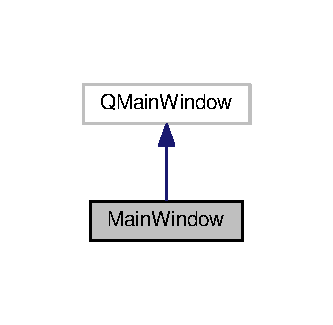
\includegraphics[width=160pt]{classMainWindow__inherit__graph}
\end{center}
\end{figure}


Collaboration diagram for Main\+Window\+:
\nopagebreak
\begin{figure}[H]
\begin{center}
\leavevmode
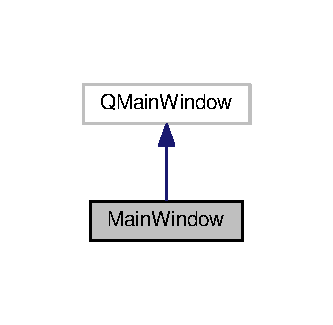
\includegraphics[width=160pt]{classMainWindow__coll__graph}
\end{center}
\end{figure}
\subsection*{Public Member Functions}
\begin{DoxyCompactItemize}
\item 
\hyperlink{classMainWindow_a8b244be8b7b7db1b08de2a2acb9409db}{Main\+Window} (Q\+Widget $\ast$parent=0)
\begin{DoxyCompactList}\small\item\em \hyperlink{classMainWindow}{Main\+Window} object default contructor. \end{DoxyCompactList}\item 
\hyperlink{classMainWindow_ae98d00a93bc118200eeef9f9bba1dba7}{$\sim$\+Main\+Window} ()
\begin{DoxyCompactList}\small\item\em \hyperlink{classMainWindow}{Main\+Window} object default destructor. \end{DoxyCompactList}\end{DoxyCompactItemize}


\subsection{Detailed Description}
\hyperlink{classMainWindow}{Main\+Window} class. 

This object is the G\+UI. 

\subsection{Constructor \& Destructor Documentation}
\index{Main\+Window@{Main\+Window}!Main\+Window@{Main\+Window}}
\index{Main\+Window@{Main\+Window}!Main\+Window@{Main\+Window}}
\subsubsection[{\texorpdfstring{Main\+Window(\+Q\+Widget $\ast$parent=0)}{MainWindow(QWidget *parent=0)}}]{\setlength{\rightskip}{0pt plus 5cm}Main\+Window\+::\+Main\+Window (
\begin{DoxyParamCaption}
\item[{Q\+Widget $\ast$}]{parent = {\ttfamily 0}}
\end{DoxyParamCaption}
)\hspace{0.3cm}{\ttfamily [explicit]}}\hypertarget{classMainWindow_a8b244be8b7b7db1b08de2a2acb9409db}{}\label{classMainWindow_a8b244be8b7b7db1b08de2a2acb9409db}


\hyperlink{classMainWindow}{Main\+Window} object default contructor. 

Initializes a \hyperlink{classMainWindow}{Main\+Window} object. \index{Main\+Window@{Main\+Window}!````~Main\+Window@{$\sim$\+Main\+Window}}
\index{````~Main\+Window@{$\sim$\+Main\+Window}!Main\+Window@{Main\+Window}}
\subsubsection[{\texorpdfstring{$\sim$\+Main\+Window()}{~MainWindow()}}]{\setlength{\rightskip}{0pt plus 5cm}Main\+Window\+::$\sim$\+Main\+Window (
\begin{DoxyParamCaption}
{}
\end{DoxyParamCaption}
)}\hypertarget{classMainWindow_ae98d00a93bc118200eeef9f9bba1dba7}{}\label{classMainWindow_ae98d00a93bc118200eeef9f9bba1dba7}


\hyperlink{classMainWindow}{Main\+Window} object default destructor. 

Destructs a \hyperlink{classMainWindow}{Main\+Window} object. 

The documentation for this class was generated from the following file\+:\begin{DoxyCompactItemize}
\item 
supercomputer/mainwindow.\+h\end{DoxyCompactItemize}

\hypertarget{classState}{}\section{State Class Reference}
\label{classState}\index{State@{State}}


\hyperlink{classState}{State} class.  




{\ttfamily \#include $<$state.\+h$>$}

\subsection*{Public Member Functions}
\begin{DoxyCompactItemize}
\item 
\hyperlink{classState_a08aed9caf1cc4d3be0ba98ec6ce361b6}{State} (long long int total\+\_\+cores, time\+\_\+t time, State\+Type state\+\_\+type)
\begin{DoxyCompactList}\small\item\em \hyperlink{classState}{State} object default contructor. \end{DoxyCompactList}\item 
\hyperlink{classState_a5c1f8c662bc19d86e5b63104b7be9a1c}{State} (\hyperlink{classState}{State} state, time\+\_\+t time, State\+Type state\+\_\+type)
\begin{DoxyCompactList}\small\item\em \hyperlink{classState}{State} object alternative contructor. \end{DoxyCompactList}\item 
void \hyperlink{classState_a576b0286b5b9bb517b45c29749f5563c}{set\+\_\+period} (time\+\_\+t start, time\+\_\+t end)
\begin{DoxyCompactList}\small\item\em Public method. Defines the period of life of a state. \end{DoxyCompactList}\item 
void \hyperlink{classState_a03e0b92997f17eed2272c67cfcdd889a}{insert\+\_\+job} (\hyperlink{classJob}{Job} job)
\begin{DoxyCompactList}\small\item\em Public method. Decreases number of available cores according to job type. \end{DoxyCompactList}\item 
bool \hyperlink{classState_a5307764c6bd8793d84b791c47e847635}{can\+\_\+insert\+\_\+job} (\hyperlink{classJob}{Job} job)
\begin{DoxyCompactList}\small\item\em Public method. Indicates whether a job can be inserted in this state or not. \end{DoxyCompactList}\item 
time\+\_\+t \hyperlink{classState_a5fa477c55eb40f020372974f84b7a5e6}{get\+\_\+time} ()
\begin{DoxyCompactList}\small\item\em Public method. Returns the state time of occurence. \end{DoxyCompactList}\item 
string \hyperlink{classState_ae179223944551fda8ffadbde68972a4f}{get\+\_\+name} ()
\begin{DoxyCompactList}\small\item\em Public method. Returns the state time of occurence. \end{DoxyCompactList}\item 
State\+Type \hyperlink{classState_a59a20bf57d4ffb9748cbf3b1c051c071}{get\+\_\+type} ()
\begin{DoxyCompactList}\small\item\em Public method. Returns type of state. \end{DoxyCompactList}\item 
long long int \hyperlink{classState_a29689f616cf6fca4c07b5a7952c324a4}{get\+\_\+short\+\_\+cores} ()
\begin{DoxyCompactList}\small\item\em Public method. Returns available number of cores reserved for short jobs. \end{DoxyCompactList}\item 
long long int \hyperlink{classState_a6f260fbc2e8cf6ffeb9249808e07c525}{get\+\_\+medium\+\_\+cores} ()
\begin{DoxyCompactList}\small\item\em Public method. Returns available number of cores reserved for medium jobs. \end{DoxyCompactList}\item 
long long int \hyperlink{classState_a97489ea52b70c2a2630ce80655c94d16}{get\+\_\+large\+\_\+cores} ()
\begin{DoxyCompactList}\small\item\em Public method. Returns available number of cores reserved for large jobs. \end{DoxyCompactList}\item 
long long int \hyperlink{classState_a3b5789fd6d375e09066b3119f994a536}{get\+\_\+total\+\_\+cores} ()
\begin{DoxyCompactList}\small\item\em Public method. Returns total number of cores. \end{DoxyCompactList}\item 
long long int \hyperlink{classState_a3be179b26f26137117e2e303d7b1bbdc}{get\+\_\+used\+\_\+cores} ()
\begin{DoxyCompactList}\small\item\em Public method. Returns total number of used cores. \end{DoxyCompactList}\end{DoxyCompactItemize}
\subsection*{Friends}
\begin{DoxyCompactItemize}
\item 
bool \hyperlink{classState_a3d174276607841e38f2c6291a46c1c8f}{operator$<$} (\hyperlink{classState}{State} const \&a, \hyperlink{classState}{State} const \&b)
\begin{DoxyCompactList}\small\item\em Operator overload. Overloads the $<$ operator according to time of ocurence. \end{DoxyCompactList}\end{DoxyCompactItemize}


\subsection{Detailed Description}
\hyperlink{classState}{State} class. 

This object represents a the number of cores available in each queue at every start time and end time of a job. 

\subsection{Constructor \& Destructor Documentation}
\index{State@{State}!State@{State}}
\index{State@{State}!State@{State}}
\subsubsection[{\texorpdfstring{State(long long int total\+\_\+cores, time\+\_\+t time, State\+Type state\+\_\+type)}{State(long long int total_cores, time_t time, StateType state_type)}}]{\setlength{\rightskip}{0pt plus 5cm}State\+::\+State (
\begin{DoxyParamCaption}
\item[{long long int}]{total\+\_\+cores, }
\item[{time\+\_\+t}]{time, }
\item[{State\+Type}]{state\+\_\+type}
\end{DoxyParamCaption}
)}\hypertarget{classState_a08aed9caf1cc4d3be0ba98ec6ce361b6}{}\label{classState_a08aed9caf1cc4d3be0ba98ec6ce361b6}


\hyperlink{classState}{State} object default contructor. 

Private time\+\_\+t. Time which this state occurs reprensented in U\+N\+IX timestamp.

Initializes a \hyperlink{classJob}{Job} object. 
\begin{DoxyParams}{Parameters}
{\em long} & long int total\+\_\+cores. Total number of system cores. \\
\hline
{\em time\+\_\+t} & time. Date of occurence. \\
\hline
{\em State\+Type} & state\+\_\+type. State\+Type indicating whether a job starts or ends.\\
\hline
\end{DoxyParams}
Default contructor of \hyperlink{classState}{State}. \index{State@{State}!State@{State}}
\index{State@{State}!State@{State}}
\subsubsection[{\texorpdfstring{State(\+State state, time\+\_\+t time, State\+Type state\+\_\+type)}{State(State state, time_t time, StateType state_type)}}]{\setlength{\rightskip}{0pt plus 5cm}State\+::\+State (
\begin{DoxyParamCaption}
\item[{{\bf State}}]{state, }
\item[{time\+\_\+t}]{time, }
\item[{State\+Type}]{state\+\_\+type}
\end{DoxyParamCaption}
)}\hypertarget{classState_a5c1f8c662bc19d86e5b63104b7be9a1c}{}\label{classState_a5c1f8c662bc19d86e5b63104b7be9a1c}


\hyperlink{classState}{State} object alternative contructor. 

Initializes a \hyperlink{classJob}{Job} object. 
\begin{DoxyParams}{Parameters}
{\em \hyperlink{classState}{State}} & state. \hyperlink{classState}{State} to copy cat. \\
\hline
{\em time\+\_\+t} & time. Date of occurence. \\
\hline
{\em State\+Type} & state\+\_\+type. State\+Type indicating whether a job starts or ends.\\
\hline
\end{DoxyParams}
Alternative contructor of \hyperlink{classState}{State}. 

\subsection{Member Function Documentation}
\index{State@{State}!can\+\_\+insert\+\_\+job@{can\+\_\+insert\+\_\+job}}
\index{can\+\_\+insert\+\_\+job@{can\+\_\+insert\+\_\+job}!State@{State}}
\subsubsection[{\texorpdfstring{can\+\_\+insert\+\_\+job(\+Job job)}{can_insert_job(Job job)}}]{\setlength{\rightskip}{0pt plus 5cm}bool State\+::can\+\_\+insert\+\_\+job (
\begin{DoxyParamCaption}
\item[{{\bf Job}}]{job}
\end{DoxyParamCaption}
)}\hypertarget{classState_a5307764c6bd8793d84b791c47e847635}{}\label{classState_a5307764c6bd8793d84b791c47e847635}


Public method. Indicates whether a job can be inserted in this state or not. 


\begin{DoxyParams}{Parameters}
{\em \hyperlink{classJob}{Job}} & job. \hyperlink{classJob}{Job} object containing information about what amount of computational resources to be decreased. \\
\hline
\end{DoxyParams}
\begin{DoxyReturn}{Returns}
bool. True if job can be inserted, false if can not.
\end{DoxyReturn}
Indicates whether a job can run with the available computational resources at this system state. \index{State@{State}!get\+\_\+large\+\_\+cores@{get\+\_\+large\+\_\+cores}}
\index{get\+\_\+large\+\_\+cores@{get\+\_\+large\+\_\+cores}!State@{State}}
\subsubsection[{\texorpdfstring{get\+\_\+large\+\_\+cores()}{get_large_cores()}}]{\setlength{\rightskip}{0pt plus 5cm}long long int State\+::get\+\_\+large\+\_\+cores (
\begin{DoxyParamCaption}
{}
\end{DoxyParamCaption}
)}\hypertarget{classState_a97489ea52b70c2a2630ce80655c94d16}{}\label{classState_a97489ea52b70c2a2630ce80655c94d16}


Public method. Returns available number of cores reserved for large jobs. 

\begin{DoxyReturn}{Returns}
ong long int. Number of cores.
\end{DoxyReturn}
Returns the amount of available computational resources for large jobs. \index{State@{State}!get\+\_\+medium\+\_\+cores@{get\+\_\+medium\+\_\+cores}}
\index{get\+\_\+medium\+\_\+cores@{get\+\_\+medium\+\_\+cores}!State@{State}}
\subsubsection[{\texorpdfstring{get\+\_\+medium\+\_\+cores()}{get_medium_cores()}}]{\setlength{\rightskip}{0pt plus 5cm}long long int State\+::get\+\_\+medium\+\_\+cores (
\begin{DoxyParamCaption}
{}
\end{DoxyParamCaption}
)}\hypertarget{classState_a6f260fbc2e8cf6ffeb9249808e07c525}{}\label{classState_a6f260fbc2e8cf6ffeb9249808e07c525}


Public method. Returns available number of cores reserved for medium jobs. 

\begin{DoxyReturn}{Returns}
ong long int. Number of cores.
\end{DoxyReturn}
Returns the amount of available computational resources for medium jobs. \index{State@{State}!get\+\_\+name@{get\+\_\+name}}
\index{get\+\_\+name@{get\+\_\+name}!State@{State}}
\subsubsection[{\texorpdfstring{get\+\_\+name()}{get_name()}}]{\setlength{\rightskip}{0pt plus 5cm}string State\+::get\+\_\+name (
\begin{DoxyParamCaption}
{}
\end{DoxyParamCaption}
)}\hypertarget{classState_ae179223944551fda8ffadbde68972a4f}{}\label{classState_ae179223944551fda8ffadbde68972a4f}


Public method. Returns the state time of occurence. 

\begin{DoxyReturn}{Returns}
time\+\_\+t. Date in U\+N\+IX timestamp. 
\end{DoxyReturn}
\index{State@{State}!get\+\_\+short\+\_\+cores@{get\+\_\+short\+\_\+cores}}
\index{get\+\_\+short\+\_\+cores@{get\+\_\+short\+\_\+cores}!State@{State}}
\subsubsection[{\texorpdfstring{get\+\_\+short\+\_\+cores()}{get_short_cores()}}]{\setlength{\rightskip}{0pt plus 5cm}long long int State\+::get\+\_\+short\+\_\+cores (
\begin{DoxyParamCaption}
{}
\end{DoxyParamCaption}
)}\hypertarget{classState_a29689f616cf6fca4c07b5a7952c324a4}{}\label{classState_a29689f616cf6fca4c07b5a7952c324a4}


Public method. Returns available number of cores reserved for short jobs. 

\begin{DoxyReturn}{Returns}
ong long int. Number of cores.
\end{DoxyReturn}
Returns the amount of available computational resources for short jobs. \index{State@{State}!get\+\_\+time@{get\+\_\+time}}
\index{get\+\_\+time@{get\+\_\+time}!State@{State}}
\subsubsection[{\texorpdfstring{get\+\_\+time()}{get_time()}}]{\setlength{\rightskip}{0pt plus 5cm}time\+\_\+t State\+::get\+\_\+time (
\begin{DoxyParamCaption}
{}
\end{DoxyParamCaption}
)}\hypertarget{classState_a5fa477c55eb40f020372974f84b7a5e6}{}\label{classState_a5fa477c55eb40f020372974f84b7a5e6}


Public method. Returns the state time of occurence. 

\begin{DoxyReturn}{Returns}
time\+\_\+t. Date in U\+N\+IX timestamp.
\end{DoxyReturn}
Returns time of ocurrence. \index{State@{State}!get\+\_\+total\+\_\+cores@{get\+\_\+total\+\_\+cores}}
\index{get\+\_\+total\+\_\+cores@{get\+\_\+total\+\_\+cores}!State@{State}}
\subsubsection[{\texorpdfstring{get\+\_\+total\+\_\+cores()}{get_total_cores()}}]{\setlength{\rightskip}{0pt plus 5cm}long long int State\+::get\+\_\+total\+\_\+cores (
\begin{DoxyParamCaption}
{}
\end{DoxyParamCaption}
)}\hypertarget{classState_a3b5789fd6d375e09066b3119f994a536}{}\label{classState_a3b5789fd6d375e09066b3119f994a536}


Public method. Returns total number of cores. 

\begin{DoxyReturn}{Returns}
ong long int. Number of cores.
\end{DoxyReturn}
Returns the total number of cores. \index{State@{State}!get\+\_\+type@{get\+\_\+type}}
\index{get\+\_\+type@{get\+\_\+type}!State@{State}}
\subsubsection[{\texorpdfstring{get\+\_\+type()}{get_type()}}]{\setlength{\rightskip}{0pt plus 5cm}State\+Type State\+::get\+\_\+type (
\begin{DoxyParamCaption}
{}
\end{DoxyParamCaption}
)}\hypertarget{classState_a59a20bf57d4ffb9748cbf3b1c051c071}{}\label{classState_a59a20bf57d4ffb9748cbf3b1c051c071}


Public method. Returns type of state. 

\begin{DoxyReturn}{Returns}
State\+Type. Start or End.
\end{DoxyReturn}
Returns state type. \index{State@{State}!get\+\_\+used\+\_\+cores@{get\+\_\+used\+\_\+cores}}
\index{get\+\_\+used\+\_\+cores@{get\+\_\+used\+\_\+cores}!State@{State}}
\subsubsection[{\texorpdfstring{get\+\_\+used\+\_\+cores()}{get_used_cores()}}]{\setlength{\rightskip}{0pt plus 5cm}long long int State\+::get\+\_\+used\+\_\+cores (
\begin{DoxyParamCaption}
{}
\end{DoxyParamCaption}
)}\hypertarget{classState_a3be179b26f26137117e2e303d7b1bbdc}{}\label{classState_a3be179b26f26137117e2e303d7b1bbdc}


Public method. Returns total number of used cores. 

\begin{DoxyReturn}{Returns}
ong long int. Number of cores.
\end{DoxyReturn}
Returns the number of used cores. \index{State@{State}!insert\+\_\+job@{insert\+\_\+job}}
\index{insert\+\_\+job@{insert\+\_\+job}!State@{State}}
\subsubsection[{\texorpdfstring{insert\+\_\+job(\+Job job)}{insert_job(Job job)}}]{\setlength{\rightskip}{0pt plus 5cm}void State\+::insert\+\_\+job (
\begin{DoxyParamCaption}
\item[{{\bf Job}}]{job}
\end{DoxyParamCaption}
)}\hypertarget{classState_a03e0b92997f17eed2272c67cfcdd889a}{}\label{classState_a03e0b92997f17eed2272c67cfcdd889a}


Public method. Decreases number of available cores according to job type. 


\begin{DoxyParams}{Parameters}
{\em \hyperlink{classJob}{Job}} & job. \hyperlink{classJob}{Job} object containing information about what amount of computational resources to be decreased.\\
\hline
\end{DoxyParams}
Decreases the available number of a computational resources available in the system according to type of job. \index{State@{State}!set\+\_\+period@{set\+\_\+period}}
\index{set\+\_\+period@{set\+\_\+period}!State@{State}}
\subsubsection[{\texorpdfstring{set\+\_\+period(time\+\_\+t start, time\+\_\+t end)}{set_period(time_t start, time_t end)}}]{\setlength{\rightskip}{0pt plus 5cm}void State\+::set\+\_\+period (
\begin{DoxyParamCaption}
\item[{time\+\_\+t}]{start, }
\item[{time\+\_\+t}]{end}
\end{DoxyParamCaption}
)}\hypertarget{classState_a576b0286b5b9bb517b45c29749f5563c}{}\label{classState_a576b0286b5b9bb517b45c29749f5563c}


Public method. Defines the period of life of a state. 


\begin{DoxyParams}{Parameters}
{\em time\+\_\+t} & start. Starting time. \\
\hline
{\em time\+\_\+t} & end. Ending time. \\
\hline
\end{DoxyParams}


\subsection{Friends And Related Function Documentation}
\index{State@{State}!operator$<$@{operator$<$}}
\index{operator$<$@{operator$<$}!State@{State}}
\subsubsection[{\texorpdfstring{operator$<$}{operator<}}]{\setlength{\rightskip}{0pt plus 5cm}bool operator$<$ (
\begin{DoxyParamCaption}
\item[{{\bf State} const \&}]{a, }
\item[{{\bf State} const \&}]{b}
\end{DoxyParamCaption}
)\hspace{0.3cm}{\ttfamily [friend]}}\hypertarget{classState_a3d174276607841e38f2c6291a46c1c8f}{}\label{classState_a3d174276607841e38f2c6291a46c1c8f}


Operator overload. Overloads the $<$ operator according to time of ocurence. 

$<$ Operator overload. 

The documentation for this class was generated from the following files\+:\begin{DoxyCompactItemize}
\item 
supercomputer/src/system/state.\+h\item 
supercomputer/src/system/state.\+cpp\end{DoxyCompactItemize}

\hypertarget{classStatistics}{}\section{Statistics Class Reference}
\label{classStatistics}\index{Statistics@{Statistics}}


\hyperlink{classStatistics}{Statistics} class.  




{\ttfamily \#include $<$statistics.\+h$>$}

\subsection*{Public Member Functions}
\begin{DoxyCompactItemize}
\item 
\hyperlink{classStatistics_abf8cd294ac6cda2aeee639defc276702}{Statistics} (\hyperlink{classConfiguration}{Configuration} $\ast$config)
\begin{DoxyCompactList}\small\item\em \hyperlink{classStatistics}{Statistics} object default contructor. \end{DoxyCompactList}\item 
string \hyperlink{classStatistics_af4c128bde8bed27787f5ecdb08bf9929}{get\+\_\+usage\+\_\+price} ()
\begin{DoxyCompactList}\small\item\em Public method. Returns the total usage price as a string. \end{DoxyCompactList}\item 
string \hyperlink{classStatistics_afb354cc8fcd9ab43ec9c3d9e2880e660}{get\+\_\+machine\+\_\+time} ()
\begin{DoxyCompactList}\small\item\em Public method. Returns the total machine time as a string. \end{DoxyCompactList}\item 
string \hyperlink{classStatistics_a091d26462ea4db2b2a6032b94ff49a31}{get\+\_\+operational\+\_\+cost} ()
\begin{DoxyCompactList}\small\item\em Public method. Returns the total operational cost as a string. \end{DoxyCompactList}\item 
string \hyperlink{classStatistics_a20e75d62f6802875eec1ebd8424d84b1}{get\+\_\+economic\+\_\+balance} ()
\begin{DoxyCompactList}\small\item\em Public method. Returns the economic balance as a string. \end{DoxyCompactList}\item 
string \hyperlink{classStatistics_a6f5e39adedce4de0c0983619fb8498c8}{get\+\_\+weekly\+\_\+usage} ()
\begin{DoxyCompactList}\small\item\em Public method. Returns the weekly usage as a string. \end{DoxyCompactList}\item 
string \hyperlink{classStatistics_a7858a6d068d7c56d29a5f54c20a8521c}{get\+\_\+short\+\_\+ta} ()
\begin{DoxyCompactList}\small\item\em Public method. Returns the average turn around ratio of short jobs. \end{DoxyCompactList}\item 
string \hyperlink{classStatistics_a114925dbd18467fed3db887104d27807}{get\+\_\+medium\+\_\+ta} ()
\begin{DoxyCompactList}\small\item\em Public method. Returns the average turn around ratio of medium jobs. \end{DoxyCompactList}\item 
string \hyperlink{classStatistics_a6f0aacba4f01c18cc9da75b1cb2f3e51}{get\+\_\+large\+\_\+ta} ()
\begin{DoxyCompactList}\small\item\em Public method. Returns the average turn around ratio of large jobs. \end{DoxyCompactList}\item 
string \hyperlink{classStatistics_a6afcfec266fe44d1c876be80f09f6de3}{get\+\_\+huge\+\_\+ta} ()
\begin{DoxyCompactList}\small\item\em Public method. Returns the average turn around ratio of huge jobs. \end{DoxyCompactList}\item 
string \hyperlink{classStatistics_abef59b8f494093e62ff1a27bd989e42a}{get\+\_\+short\+\_\+wt} ()
\begin{DoxyCompactList}\small\item\em Public method. Returns the average waiting time of short jobs. \end{DoxyCompactList}\item 
string \hyperlink{classStatistics_aa20489eecdafe0ebcac554f34b60caef}{get\+\_\+medium\+\_\+wt} ()
\begin{DoxyCompactList}\small\item\em Public method. Returns the average waiting time of medium jobs. \end{DoxyCompactList}\item 
string \hyperlink{classStatistics_a06c13d01f1a8ea83391628b9bf617a4f}{get\+\_\+large\+\_\+wt} ()
\begin{DoxyCompactList}\small\item\em Public method. Returns the average waiting time of large jobs. \end{DoxyCompactList}\item 
string \hyperlink{classStatistics_a17dc31579326d8463eba7dd661673f47}{get\+\_\+huge\+\_\+wt} ()
\begin{DoxyCompactList}\small\item\em Public method. Returns the average waiting time of huge jobs. \end{DoxyCompactList}\item 
void \hyperlink{classStatistics_af99eab950e1fa1a657332fface5dc13e}{add\+\_\+usage\+\_\+price} (double price)
\begin{DoxyCompactList}\small\item\em Public method. Adds price to total usage price. \end{DoxyCompactList}\item 
void \hyperlink{classStatistics_a17bca1fa9938f98e93cebd56d428f9a4}{add\+\_\+operational\+\_\+cost} (double cost)
\begin{DoxyCompactList}\small\item\em Public method. Adds cost to total operational cost. \end{DoxyCompactList}\item 
void \hyperlink{classStatistics_a726b0734f8a0c86024543190ab3092ea}{add\+\_\+machine\+\_\+time} (unsigned long long int time)
\begin{DoxyCompactList}\small\item\em Public method. Adds time to total machine time. \end{DoxyCompactList}\item 
void \hyperlink{classStatistics_a78e4c255a4999ebd6c8872eef6360427}{add\+\_\+job} (time\+\_\+t start, \hyperlink{classJob}{Job} job)
\begin{DoxyCompactList}\small\item\em Public method. Adds job to waiting time and turn around vectors. \end{DoxyCompactList}\end{DoxyCompactItemize}


\subsection{Detailed Description}
\hyperlink{classStatistics}{Statistics} class. 

This object keeps statistics information structured and organized. 

\subsection{Constructor \& Destructor Documentation}
\index{Statistics@{Statistics}!Statistics@{Statistics}}
\index{Statistics@{Statistics}!Statistics@{Statistics}}
\subsubsection[{\texorpdfstring{Statistics(\+Configuration $\ast$config)}{Statistics(Configuration *config)}}]{\setlength{\rightskip}{0pt plus 5cm}Statistics\+::\+Statistics (
\begin{DoxyParamCaption}
\item[{{\bf Configuration} $\ast$}]{config}
\end{DoxyParamCaption}
)}\hypertarget{classStatistics_abf8cd294ac6cda2aeee639defc276702}{}\label{classStatistics_abf8cd294ac6cda2aeee639defc276702}


\hyperlink{classStatistics}{Statistics} object default contructor. 

Private unsigned long long int. Total machine time of the simulation.

Initializes a \hyperlink{classStatistics}{Statistics} object. 
\begin{DoxyParams}{Parameters}
{\em Configuration$\ast$} & config. Defines which configuration this statistics object should follow.\\
\hline
\end{DoxyParams}
Contructor of \hyperlink{classStatistics}{Statistics} object. 

\subsection{Member Function Documentation}
\index{Statistics@{Statistics}!add\+\_\+job@{add\+\_\+job}}
\index{add\+\_\+job@{add\+\_\+job}!Statistics@{Statistics}}
\subsubsection[{\texorpdfstring{add\+\_\+job(time\+\_\+t start, Job job)}{add_job(time_t start, Job job)}}]{\setlength{\rightskip}{0pt plus 5cm}void Statistics\+::add\+\_\+job (
\begin{DoxyParamCaption}
\item[{time\+\_\+t}]{start, }
\item[{{\bf Job}}]{job}
\end{DoxyParamCaption}
)}\hypertarget{classStatistics_a78e4c255a4999ebd6c8872eef6360427}{}\label{classStatistics_a78e4c255a4999ebd6c8872eef6360427}


Public method. Adds job to waiting time and turn around vectors. 


\begin{DoxyParams}{Parameters}
{\em time\+\_\+t} & start. Time of start. \\
\hline
{\em \hyperlink{classJob}{Job}} & job. \hyperlink{classJob}{Job} to be added.\\
\hline
\end{DoxyParams}
Adds job to waiting time and turn around ratio vectors according to its type. Increments the number of Short, Medium, Large or Huge jobs processed in the week of job start time. \index{Statistics@{Statistics}!add\+\_\+machine\+\_\+time@{add\+\_\+machine\+\_\+time}}
\index{add\+\_\+machine\+\_\+time@{add\+\_\+machine\+\_\+time}!Statistics@{Statistics}}
\subsubsection[{\texorpdfstring{add\+\_\+machine\+\_\+time(unsigned long long int time)}{add_machine_time(unsigned long long int time)}}]{\setlength{\rightskip}{0pt plus 5cm}void Statistics\+::add\+\_\+machine\+\_\+time (
\begin{DoxyParamCaption}
\item[{unsigned long long int}]{time}
\end{DoxyParamCaption}
)}\hypertarget{classStatistics_a726b0734f8a0c86024543190ab3092ea}{}\label{classStatistics_a726b0734f8a0c86024543190ab3092ea}


Public method. Adds time to total machine time. 


\begin{DoxyParams}{Parameters}
{\em unsigned} & long long int time. Time in seconds to be added.\\
\hline
\end{DoxyParams}
Adds time to system total machine time. \index{Statistics@{Statistics}!add\+\_\+operational\+\_\+cost@{add\+\_\+operational\+\_\+cost}}
\index{add\+\_\+operational\+\_\+cost@{add\+\_\+operational\+\_\+cost}!Statistics@{Statistics}}
\subsubsection[{\texorpdfstring{add\+\_\+operational\+\_\+cost(double cost)}{add_operational_cost(double cost)}}]{\setlength{\rightskip}{0pt plus 5cm}void Statistics\+::add\+\_\+operational\+\_\+cost (
\begin{DoxyParamCaption}
\item[{double}]{cost}
\end{DoxyParamCaption}
)}\hypertarget{classStatistics_a17bca1fa9938f98e93cebd56d428f9a4}{}\label{classStatistics_a17bca1fa9938f98e93cebd56d428f9a4}


Public method. Adds cost to total operational cost. 


\begin{DoxyParams}{Parameters}
{\em double} & cost. Cost to be added.\\
\hline
\end{DoxyParams}
Adds operational cost to system total operational cost. \index{Statistics@{Statistics}!add\+\_\+usage\+\_\+price@{add\+\_\+usage\+\_\+price}}
\index{add\+\_\+usage\+\_\+price@{add\+\_\+usage\+\_\+price}!Statistics@{Statistics}}
\subsubsection[{\texorpdfstring{add\+\_\+usage\+\_\+price(double price)}{add_usage_price(double price)}}]{\setlength{\rightskip}{0pt plus 5cm}void Statistics\+::add\+\_\+usage\+\_\+price (
\begin{DoxyParamCaption}
\item[{double}]{price}
\end{DoxyParamCaption}
)}\hypertarget{classStatistics_af99eab950e1fa1a657332fface5dc13e}{}\label{classStatistics_af99eab950e1fa1a657332fface5dc13e}


Public method. Adds price to total usage price. 


\begin{DoxyParams}{Parameters}
{\em double} & price. Price to be added.\\
\hline
\end{DoxyParams}
Adds usage price to system total usage price. \index{Statistics@{Statistics}!get\+\_\+economic\+\_\+balance@{get\+\_\+economic\+\_\+balance}}
\index{get\+\_\+economic\+\_\+balance@{get\+\_\+economic\+\_\+balance}!Statistics@{Statistics}}
\subsubsection[{\texorpdfstring{get\+\_\+economic\+\_\+balance()}{get_economic_balance()}}]{\setlength{\rightskip}{0pt plus 5cm}string Statistics\+::get\+\_\+economic\+\_\+balance (
\begin{DoxyParamCaption}
{}
\end{DoxyParamCaption}
)}\hypertarget{classStatistics_a20e75d62f6802875eec1ebd8424d84b1}{}\label{classStatistics_a20e75d62f6802875eec1ebd8424d84b1}


Public method. Returns the economic balance as a string. 

\begin{DoxyReturn}{Returns}
string. Economic balance string.
\end{DoxyReturn}
Returns system economic balance as a string with a precision of 2 decimal places. \index{Statistics@{Statistics}!get\+\_\+huge\+\_\+ta@{get\+\_\+huge\+\_\+ta}}
\index{get\+\_\+huge\+\_\+ta@{get\+\_\+huge\+\_\+ta}!Statistics@{Statistics}}
\subsubsection[{\texorpdfstring{get\+\_\+huge\+\_\+ta()}{get_huge_ta()}}]{\setlength{\rightskip}{0pt plus 5cm}string Statistics\+::get\+\_\+huge\+\_\+ta (
\begin{DoxyParamCaption}
{}
\end{DoxyParamCaption}
)}\hypertarget{classStatistics_a6afcfec266fe44d1c876be80f09f6de3}{}\label{classStatistics_a6afcfec266fe44d1c876be80f09f6de3}


Public method. Returns the average turn around ratio of huge jobs. 

\begin{DoxyReturn}{Returns}
string. Turn around ratio of huge jobs string.
\end{DoxyReturn}
Returns average of turn around times of huge jobs as a string with a precision of 2 decimal places. \index{Statistics@{Statistics}!get\+\_\+huge\+\_\+wt@{get\+\_\+huge\+\_\+wt}}
\index{get\+\_\+huge\+\_\+wt@{get\+\_\+huge\+\_\+wt}!Statistics@{Statistics}}
\subsubsection[{\texorpdfstring{get\+\_\+huge\+\_\+wt()}{get_huge_wt()}}]{\setlength{\rightskip}{0pt plus 5cm}string Statistics\+::get\+\_\+huge\+\_\+wt (
\begin{DoxyParamCaption}
{}
\end{DoxyParamCaption}
)}\hypertarget{classStatistics_a17dc31579326d8463eba7dd661673f47}{}\label{classStatistics_a17dc31579326d8463eba7dd661673f47}


Public method. Returns the average waiting time of huge jobs. 

\begin{DoxyReturn}{Returns}
string. Average waiting time of huge jobs string.
\end{DoxyReturn}
Returns average of waiting times of huge jobs as a string with a precision of 2 decimal places. \index{Statistics@{Statistics}!get\+\_\+large\+\_\+ta@{get\+\_\+large\+\_\+ta}}
\index{get\+\_\+large\+\_\+ta@{get\+\_\+large\+\_\+ta}!Statistics@{Statistics}}
\subsubsection[{\texorpdfstring{get\+\_\+large\+\_\+ta()}{get_large_ta()}}]{\setlength{\rightskip}{0pt plus 5cm}string Statistics\+::get\+\_\+large\+\_\+ta (
\begin{DoxyParamCaption}
{}
\end{DoxyParamCaption}
)}\hypertarget{classStatistics_a6f0aacba4f01c18cc9da75b1cb2f3e51}{}\label{classStatistics_a6f0aacba4f01c18cc9da75b1cb2f3e51}


Public method. Returns the average turn around ratio of large jobs. 

\begin{DoxyReturn}{Returns}
string. Turn around ratio of large jobs string.
\end{DoxyReturn}
Returns average of turn around times of large jobs as a string with a precision of 2 decimal places. \index{Statistics@{Statistics}!get\+\_\+large\+\_\+wt@{get\+\_\+large\+\_\+wt}}
\index{get\+\_\+large\+\_\+wt@{get\+\_\+large\+\_\+wt}!Statistics@{Statistics}}
\subsubsection[{\texorpdfstring{get\+\_\+large\+\_\+wt()}{get_large_wt()}}]{\setlength{\rightskip}{0pt plus 5cm}string Statistics\+::get\+\_\+large\+\_\+wt (
\begin{DoxyParamCaption}
{}
\end{DoxyParamCaption}
)}\hypertarget{classStatistics_a06c13d01f1a8ea83391628b9bf617a4f}{}\label{classStatistics_a06c13d01f1a8ea83391628b9bf617a4f}


Public method. Returns the average waiting time of large jobs. 

\begin{DoxyReturn}{Returns}
string. Average waiting time of large jobs string.
\end{DoxyReturn}
Returns average of waiting times of large jobs as a string with a precision of 2 decimal places. \index{Statistics@{Statistics}!get\+\_\+machine\+\_\+time@{get\+\_\+machine\+\_\+time}}
\index{get\+\_\+machine\+\_\+time@{get\+\_\+machine\+\_\+time}!Statistics@{Statistics}}
\subsubsection[{\texorpdfstring{get\+\_\+machine\+\_\+time()}{get_machine_time()}}]{\setlength{\rightskip}{0pt plus 5cm}string Statistics\+::get\+\_\+machine\+\_\+time (
\begin{DoxyParamCaption}
{}
\end{DoxyParamCaption}
)}\hypertarget{classStatistics_afb354cc8fcd9ab43ec9c3d9e2880e660}{}\label{classStatistics_afb354cc8fcd9ab43ec9c3d9e2880e660}


Public method. Returns the total machine time as a string. 

\begin{DoxyReturn}{Returns}
string. Machine time string.
\end{DoxyReturn}
Returns the machine time as a string with the number of days, hours, minutes and seconds. \index{Statistics@{Statistics}!get\+\_\+medium\+\_\+ta@{get\+\_\+medium\+\_\+ta}}
\index{get\+\_\+medium\+\_\+ta@{get\+\_\+medium\+\_\+ta}!Statistics@{Statistics}}
\subsubsection[{\texorpdfstring{get\+\_\+medium\+\_\+ta()}{get_medium_ta()}}]{\setlength{\rightskip}{0pt plus 5cm}string Statistics\+::get\+\_\+medium\+\_\+ta (
\begin{DoxyParamCaption}
{}
\end{DoxyParamCaption}
)}\hypertarget{classStatistics_a114925dbd18467fed3db887104d27807}{}\label{classStatistics_a114925dbd18467fed3db887104d27807}


Public method. Returns the average turn around ratio of medium jobs. 

\begin{DoxyReturn}{Returns}
string. Turn around ratio of medium jobs string.
\end{DoxyReturn}
Returns average of turn around times of medium jobs as a string with a precision of 2 decimal places. \index{Statistics@{Statistics}!get\+\_\+medium\+\_\+wt@{get\+\_\+medium\+\_\+wt}}
\index{get\+\_\+medium\+\_\+wt@{get\+\_\+medium\+\_\+wt}!Statistics@{Statistics}}
\subsubsection[{\texorpdfstring{get\+\_\+medium\+\_\+wt()}{get_medium_wt()}}]{\setlength{\rightskip}{0pt plus 5cm}string Statistics\+::get\+\_\+medium\+\_\+wt (
\begin{DoxyParamCaption}
{}
\end{DoxyParamCaption}
)}\hypertarget{classStatistics_aa20489eecdafe0ebcac554f34b60caef}{}\label{classStatistics_aa20489eecdafe0ebcac554f34b60caef}


Public method. Returns the average waiting time of medium jobs. 

\begin{DoxyReturn}{Returns}
string. Average waiting time of medium jobs string.
\end{DoxyReturn}
Returns average of waiting times of medium jobs as a string with a precision of 2 decimal places. \index{Statistics@{Statistics}!get\+\_\+operational\+\_\+cost@{get\+\_\+operational\+\_\+cost}}
\index{get\+\_\+operational\+\_\+cost@{get\+\_\+operational\+\_\+cost}!Statistics@{Statistics}}
\subsubsection[{\texorpdfstring{get\+\_\+operational\+\_\+cost()}{get_operational_cost()}}]{\setlength{\rightskip}{0pt plus 5cm}string Statistics\+::get\+\_\+operational\+\_\+cost (
\begin{DoxyParamCaption}
{}
\end{DoxyParamCaption}
)}\hypertarget{classStatistics_a091d26462ea4db2b2a6032b94ff49a31}{}\label{classStatistics_a091d26462ea4db2b2a6032b94ff49a31}


Public method. Returns the total operational cost as a string. 

\begin{DoxyReturn}{Returns}
string. Operational cost string.
\end{DoxyReturn}
Returns system total operational cost as a string with a precision of 2 decimal places. \index{Statistics@{Statistics}!get\+\_\+short\+\_\+ta@{get\+\_\+short\+\_\+ta}}
\index{get\+\_\+short\+\_\+ta@{get\+\_\+short\+\_\+ta}!Statistics@{Statistics}}
\subsubsection[{\texorpdfstring{get\+\_\+short\+\_\+ta()}{get_short_ta()}}]{\setlength{\rightskip}{0pt plus 5cm}string Statistics\+::get\+\_\+short\+\_\+ta (
\begin{DoxyParamCaption}
{}
\end{DoxyParamCaption}
)}\hypertarget{classStatistics_a7858a6d068d7c56d29a5f54c20a8521c}{}\label{classStatistics_a7858a6d068d7c56d29a5f54c20a8521c}


Public method. Returns the average turn around ratio of short jobs. 

\begin{DoxyReturn}{Returns}
string. Turn around ratio of short jobs string.
\end{DoxyReturn}
Returns average of turn around times of short jobs as a string with a precision of 2 decimal places. \index{Statistics@{Statistics}!get\+\_\+short\+\_\+wt@{get\+\_\+short\+\_\+wt}}
\index{get\+\_\+short\+\_\+wt@{get\+\_\+short\+\_\+wt}!Statistics@{Statistics}}
\subsubsection[{\texorpdfstring{get\+\_\+short\+\_\+wt()}{get_short_wt()}}]{\setlength{\rightskip}{0pt plus 5cm}string Statistics\+::get\+\_\+short\+\_\+wt (
\begin{DoxyParamCaption}
{}
\end{DoxyParamCaption}
)}\hypertarget{classStatistics_abef59b8f494093e62ff1a27bd989e42a}{}\label{classStatistics_abef59b8f494093e62ff1a27bd989e42a}


Public method. Returns the average waiting time of short jobs. 

\begin{DoxyReturn}{Returns}
string. Average waiting time of short jobs string.
\end{DoxyReturn}
Returns average of waiting times of short jobs as a string with a precision of 2 decimal places. \index{Statistics@{Statistics}!get\+\_\+usage\+\_\+price@{get\+\_\+usage\+\_\+price}}
\index{get\+\_\+usage\+\_\+price@{get\+\_\+usage\+\_\+price}!Statistics@{Statistics}}
\subsubsection[{\texorpdfstring{get\+\_\+usage\+\_\+price()}{get_usage_price()}}]{\setlength{\rightskip}{0pt plus 5cm}string Statistics\+::get\+\_\+usage\+\_\+price (
\begin{DoxyParamCaption}
{}
\end{DoxyParamCaption}
)}\hypertarget{classStatistics_af4c128bde8bed27787f5ecdb08bf9929}{}\label{classStatistics_af4c128bde8bed27787f5ecdb08bf9929}


Public method. Returns the total usage price as a string. 

\begin{DoxyReturn}{Returns}
string. Usage price string.
\end{DoxyReturn}
Returns system total usage price as a string with a precision of 2 decimal places. \index{Statistics@{Statistics}!get\+\_\+weekly\+\_\+usage@{get\+\_\+weekly\+\_\+usage}}
\index{get\+\_\+weekly\+\_\+usage@{get\+\_\+weekly\+\_\+usage}!Statistics@{Statistics}}
\subsubsection[{\texorpdfstring{get\+\_\+weekly\+\_\+usage()}{get_weekly_usage()}}]{\setlength{\rightskip}{0pt plus 5cm}string Statistics\+::get\+\_\+weekly\+\_\+usage (
\begin{DoxyParamCaption}
{}
\end{DoxyParamCaption}
)}\hypertarget{classStatistics_a6f5e39adedce4de0c0983619fb8498c8}{}\label{classStatistics_a6f5e39adedce4de0c0983619fb8498c8}


Public method. Returns the weekly usage as a string. 

\begin{DoxyReturn}{Returns}
string. \hyperlink{classSystem}{System} weekly usage.
\end{DoxyReturn}
Returns system weekly usage as a string. 

The documentation for this class was generated from the following files\+:\begin{DoxyCompactItemize}
\item 
supercomputer/src/statistics/statistics.\+h\item 
supercomputer/src/statistics/statistics.\+cpp\end{DoxyCompactItemize}

\hypertarget{classSystem}{}\section{System Class Reference}
\label{classSystem}\index{System@{System}}


\hyperlink{classSystem}{System} class.  




{\ttfamily \#include $<$system.\+h$>$}

\subsection*{Public Member Functions}
\begin{DoxyCompactItemize}
\item 
\hyperlink{classSystem_a38c393cf990b65c13bf926c6e25c4f0a}{System} (\hyperlink{classConfiguration}{Configuration} $\ast$config)
\begin{DoxyCompactList}\small\item\em \hyperlink{classSystem}{System} object default contructor. \end{DoxyCompactList}\item 
\hyperlink{classSystem_a4d2006a8a392e1c198fb988a7d125ac8}{System} (\hyperlink{classConfiguration}{Configuration} $\ast$config, vector$<$ \hyperlink{classUser}{User} $\ast$ $>$ users, vector$<$ \hyperlink{classJob}{Job} $>$ jobs)
\begin{DoxyCompactList}\small\item\em \hyperlink{classSystem}{System} object contructor for custom tests. \end{DoxyCompactList}\item 
string \hyperlink{classSystem_adbb7e0745a7a25f8a598eaa6b04dd4ed}{get\+\_\+results} ()
\begin{DoxyCompactList}\small\item\em Public method. Fetchs results of statistics object, returning a string with a specific format. \end{DoxyCompactList}\end{DoxyCompactItemize}


\subsection{Detailed Description}
\hyperlink{classSystem}{System} class. 

This object represents the computing system. 

\subsection{Constructor \& Destructor Documentation}
\index{System@{System}!System@{System}}
\index{System@{System}!System@{System}}
\subsubsection[{\texorpdfstring{System(\+Configuration $\ast$config)}{System(Configuration *config)}}]{\setlength{\rightskip}{0pt plus 5cm}System\+::\+System (
\begin{DoxyParamCaption}
\item[{{\bf Configuration} $\ast$}]{config}
\end{DoxyParamCaption}
)}\hypertarget{classSystem_a38c393cf990b65c13bf926c6e25c4f0a}{}\label{classSystem_a38c393cf990b65c13bf926c6e25c4f0a}


\hyperlink{classSystem}{System} object default contructor. 

Initializes a \hyperlink{classSystem}{System} object. 
\begin{DoxyParams}{Parameters}
{\em \hyperlink{classConfiguration}{Configuration}} & $\ast$ config. \hyperlink{classConfiguration}{Configuration} to be followed by the simulation.\\
\hline
\end{DoxyParams}
Default contructor of \hyperlink{classSystem}{System} object. Populates vector of users and jobs. Runs the scheduler algorithm and calculates the operating cost of the system. \index{System@{System}!System@{System}}
\index{System@{System}!System@{System}}
\subsubsection[{\texorpdfstring{System(\+Configuration $\ast$config, vector$<$ User $\ast$ $>$ users, vector$<$ Job $>$ jobs)}{System(Configuration *config, vector< User * > users, vector< Job > jobs)}}]{\setlength{\rightskip}{0pt plus 5cm}System\+::\+System (
\begin{DoxyParamCaption}
\item[{{\bf Configuration} $\ast$}]{config, }
\item[{vector$<$ {\bf User} $\ast$ $>$}]{users, }
\item[{vector$<$ {\bf Job} $>$}]{jobs}
\end{DoxyParamCaption}
)}\hypertarget{classSystem_a4d2006a8a392e1c198fb988a7d125ac8}{}\label{classSystem_a4d2006a8a392e1c198fb988a7d125ac8}


\hyperlink{classSystem}{System} object contructor for custom tests. 

Initializes a \hyperlink{classSystem}{System} object. 
\begin{DoxyParams}{Parameters}
{\em \hyperlink{classConfiguration}{Configuration}} & $\ast$ config. \hyperlink{classConfiguration}{Configuration} to be followed by the simulation. \\
\hline
{\em vector$<$\+User$\ast$$>$} & users. Simulated users vector. \\
\hline
{\em vector$<$\+Job$>$} & jobs. Simulated jobs vector.\\
\hline
\end{DoxyParams}
Alternative contructor of \hyperlink{classSystem}{System} object, indicated for testing purposes. Runs the scheduler algorithm and calculates the operating cost of the system. 

\subsection{Member Function Documentation}
\index{System@{System}!get\+\_\+results@{get\+\_\+results}}
\index{get\+\_\+results@{get\+\_\+results}!System@{System}}
\subsubsection[{\texorpdfstring{get\+\_\+results()}{get_results()}}]{\setlength{\rightskip}{0pt plus 5cm}string System\+::get\+\_\+results (
\begin{DoxyParamCaption}
{}
\end{DoxyParamCaption}
)}\hypertarget{classSystem_adbb7e0745a7a25f8a598eaa6b04dd4ed}{}\label{classSystem_adbb7e0745a7a25f8a598eaa6b04dd4ed}


Public method. Fetchs results of statistics object, returning a string with a specific format. 

\begin{DoxyReturn}{Returns}
string. String with information about the outputs of the simulation.
\end{DoxyReturn}
Returns string with informations about the outputs of the simulation. 

The documentation for this class was generated from the following files\+:\begin{DoxyCompactItemize}
\item 
supercomputer/src/system/system.\+h\item 
supercomputer/src/system/system.\+cpp\end{DoxyCompactItemize}

\hypertarget{classUser}{}\section{User Class Reference}
\label{classUser}\index{User@{User}}


\hyperlink{classSystem}{System} class.  




{\ttfamily \#include $<$user.\+h$>$}

\subsection*{Public Member Functions}
\begin{DoxyCompactItemize}
\item 
\hyperlink{classUser_a9ee57fd1e1dca94a043ad0f5a99ac2be}{User} (\hyperlink{classConfiguration}{Configuration} $\ast$config, int id, bool support)
\begin{DoxyCompactList}\small\item\em \hyperlink{classUser}{User} object default contructor. \end{DoxyCompactList}\item 
bool \hyperlink{classUser_a256c7f780ea27a728b2bf391e0925728}{can\+\_\+afford} (\hyperlink{classJob}{Job} $\ast$job)
\begin{DoxyCompactList}\small\item\em Public method. Method to check if an \hyperlink{classUser}{User} can afford to run a given job. \end{DoxyCompactList}\item 
void \hyperlink{classUser_ab960fea4dd1f6ea2439e410fb8cfd9bc}{pay} (\hyperlink{classJob}{Job} $\ast$job)
\begin{DoxyCompactList}\small\item\em Public method. Decreases the user budget according to the price of a job. \end{DoxyCompactList}\end{DoxyCompactItemize}


\subsection{Detailed Description}
\hyperlink{classSystem}{System} class. 

This object represents a simulated user. 

\subsection{Constructor \& Destructor Documentation}
\index{User@{User}!User@{User}}
\index{User@{User}!User@{User}}
\subsubsection[{\texorpdfstring{User(\+Configuration $\ast$config, int id, bool support)}{User(Configuration *config, int id, bool support)}}]{\setlength{\rightskip}{0pt plus 5cm}User\+::\+User (
\begin{DoxyParamCaption}
\item[{{\bf Configuration} $\ast$}]{config, }
\item[{int}]{id, }
\item[{bool}]{support}
\end{DoxyParamCaption}
)}\hypertarget{classUser_a9ee57fd1e1dca94a043ad0f5a99ac2be}{}\label{classUser_a9ee57fd1e1dca94a043ad0f5a99ac2be}


\hyperlink{classUser}{User} object default contructor. 

Initializes a \hyperlink{classUser}{User} object. 
\begin{DoxyParams}{Parameters}
{\em \hyperlink{classConfiguration}{Configuration}} & $\ast$ config. \hyperlink{classConfiguration}{Configuration} to be followed by the simulation. \\
\hline
{\em int} & id. \hyperlink{classUser}{User} id, this value is unique between users. \\
\hline
{\em bool} & support. The user is part of the IT Support if true.\\
\hline
\end{DoxyParams}
Default contructor of \hyperlink{classUser}{User}. 

\subsection{Member Function Documentation}
\index{User@{User}!can\+\_\+afford@{can\+\_\+afford}}
\index{can\+\_\+afford@{can\+\_\+afford}!User@{User}}
\subsubsection[{\texorpdfstring{can\+\_\+afford(\+Job $\ast$job)}{can_afford(Job *job)}}]{\setlength{\rightskip}{0pt plus 5cm}bool User\+::can\+\_\+afford (
\begin{DoxyParamCaption}
\item[{{\bf Job} $\ast$}]{job}
\end{DoxyParamCaption}
)}\hypertarget{classUser_a256c7f780ea27a728b2bf391e0925728}{}\label{classUser_a256c7f780ea27a728b2bf391e0925728}


Public method. Method to check if an \hyperlink{classUser}{User} can afford to run a given job. 


\begin{DoxyParams}{Parameters}
{\em \hyperlink{classJob}{Job}} & $\ast$ job. \hyperlink{classJob}{Job} to be paid. \\
\hline
\end{DoxyParams}
\begin{DoxyReturn}{Returns}
bool. True if user can afford the job, false if not.
\end{DoxyReturn}
Method to check if an user can afford for a given job. \index{User@{User}!pay@{pay}}
\index{pay@{pay}!User@{User}}
\subsubsection[{\texorpdfstring{pay(\+Job $\ast$job)}{pay(Job *job)}}]{\setlength{\rightskip}{0pt plus 5cm}void User\+::pay (
\begin{DoxyParamCaption}
\item[{{\bf Job} $\ast$}]{job}
\end{DoxyParamCaption}
)}\hypertarget{classUser_ab960fea4dd1f6ea2439e410fb8cfd9bc}{}\label{classUser_ab960fea4dd1f6ea2439e410fb8cfd9bc}


Public method. Decreases the user budget according to the price of a job. 


\begin{DoxyParams}{Parameters}
{\em \hyperlink{classJob}{Job}} & $\ast$ job. \hyperlink{classJob}{Job} to be paid.\\
\hline
\end{DoxyParams}
Method to decrease the user budget, according to the price of a given job. 

The documentation for this class was generated from the following files\+:\begin{DoxyCompactItemize}
\item 
supercomputer/src/users/user.\+h\item 
supercomputer/src/users/user.\+cpp\end{DoxyCompactItemize}

\hypertarget{classWeek}{}\section{Week Class Reference}
\label{classWeek}\index{Week@{Week}}


\hyperlink{classWeek}{Week} class.  




{\ttfamily \#include $<$week.\+h$>$}

\subsection*{Public Member Functions}
\begin{DoxyCompactItemize}
\item 
\hyperlink{classWeek_acde62b92be9795ba306655c67cb73657}{Week} (time\+\_\+t start, time\+\_\+t end)
\begin{DoxyCompactList}\small\item\em \hyperlink{classWeek}{Week} object default contructor. \end{DoxyCompactList}\item 
time\+\_\+t \hyperlink{classWeek_a09c3311872e50cc72900c97f5b2bde46}{get\+\_\+start} ()
\begin{DoxyCompactList}\small\item\em Public method. Returns the starting date of a job. \end{DoxyCompactList}\item 
time\+\_\+t \hyperlink{classWeek_a9bc75154f4fab7823f0ea9e04a69296d}{get\+\_\+end} ()
\begin{DoxyCompactList}\small\item\em Public method. Returns the ending date of a job. \end{DoxyCompactList}\item 
void \hyperlink{classWeek_a583625ac54cdbf5b38caf23c8b76ae37}{set\+\_\+start} (time\+\_\+t start)
\begin{DoxyCompactList}\small\item\em Public method. Defines new starting date of a week. \end{DoxyCompactList}\item 
void \hyperlink{classWeek_ac5f28e3ca4f43b4c4d78f9a4e140c207}{add\+\_\+job} (\hyperlink{classJob}{Job} job)
\begin{DoxyCompactList}\small\item\em Public method. Defines new starting date of a week. \end{DoxyCompactList}\end{DoxyCompactItemize}
\subsection*{Friends}
\begin{DoxyCompactItemize}
\item 
ostream \& \hyperlink{classWeek_a5c17f115d399c08f1b848e8d8ce05e3f}{operator$<$$<$} (ostream \&os, const \hyperlink{classWeek}{Week} \&week)
\begin{DoxyCompactList}\small\item\em Operator overload. Overloads the $<$$<$ operator of a \hyperlink{classWeek}{Week} object. \end{DoxyCompactList}\end{DoxyCompactItemize}


\subsection{Detailed Description}
\hyperlink{classWeek}{Week} class. 

This object keeps information about number of jobs processed in a week by each queue. 

\subsection{Constructor \& Destructor Documentation}
\index{Week@{Week}!Week@{Week}}
\index{Week@{Week}!Week@{Week}}
\subsubsection[{\texorpdfstring{Week(time\+\_\+t start, time\+\_\+t end)}{Week(time_t start, time_t end)}}]{\setlength{\rightskip}{0pt plus 5cm}Week\+::\+Week (
\begin{DoxyParamCaption}
\item[{time\+\_\+t}]{start, }
\item[{time\+\_\+t}]{end}
\end{DoxyParamCaption}
)}\hypertarget{classWeek_acde62b92be9795ba306655c67cb73657}{}\label{classWeek_acde62b92be9795ba306655c67cb73657}


\hyperlink{classWeek}{Week} object default contructor. 

Private unsigned int. Number of huge jobs processed.

Initializes a \hyperlink{classWeek}{Week} object. 
\begin{DoxyParams}{Parameters}
{\em time\+\_\+t} & start. Defines the stating date of the week. \\
\hline
{\em time\+\_\+t} & end. Defines the ending date of the week.\\
\hline
\end{DoxyParams}
Contructor of \hyperlink{classWeek}{Week} object. 

\subsection{Member Function Documentation}
\index{Week@{Week}!add\+\_\+job@{add\+\_\+job}}
\index{add\+\_\+job@{add\+\_\+job}!Week@{Week}}
\subsubsection[{\texorpdfstring{add\+\_\+job(\+Job job)}{add_job(Job job)}}]{\setlength{\rightskip}{0pt plus 5cm}void Week\+::add\+\_\+job (
\begin{DoxyParamCaption}
\item[{{\bf Job}}]{job}
\end{DoxyParamCaption}
)}\hypertarget{classWeek_ac5f28e3ca4f43b4c4d78f9a4e140c207}{}\label{classWeek_ac5f28e3ca4f43b4c4d78f9a4e140c207}


Public method. Defines new starting date of a week. 


\begin{DoxyParams}{Parameters}
{\em time\+\_\+t} & start. Starting date represented in U\+N\+IX timestamp.\\
\hline
\end{DoxyParams}
Increments the number of jobs processed this week according to its type. \index{Week@{Week}!get\+\_\+end@{get\+\_\+end}}
\index{get\+\_\+end@{get\+\_\+end}!Week@{Week}}
\subsubsection[{\texorpdfstring{get\+\_\+end()}{get_end()}}]{\setlength{\rightskip}{0pt plus 5cm}time\+\_\+t Week\+::get\+\_\+end (
\begin{DoxyParamCaption}
{}
\end{DoxyParamCaption}
)}\hypertarget{classWeek_a9bc75154f4fab7823f0ea9e04a69296d}{}\label{classWeek_a9bc75154f4fab7823f0ea9e04a69296d}


Public method. Returns the ending date of a job. 

\begin{DoxyReturn}{Returns}
time\+\_\+t. Date represented in U\+N\+IX timestamp.
\end{DoxyReturn}
Ŕeturns the ending time of a week. \index{Week@{Week}!get\+\_\+start@{get\+\_\+start}}
\index{get\+\_\+start@{get\+\_\+start}!Week@{Week}}
\subsubsection[{\texorpdfstring{get\+\_\+start()}{get_start()}}]{\setlength{\rightskip}{0pt plus 5cm}time\+\_\+t Week\+::get\+\_\+start (
\begin{DoxyParamCaption}
{}
\end{DoxyParamCaption}
)}\hypertarget{classWeek_a09c3311872e50cc72900c97f5b2bde46}{}\label{classWeek_a09c3311872e50cc72900c97f5b2bde46}


Public method. Returns the starting date of a job. 

\begin{DoxyReturn}{Returns}
time\+\_\+t. Date represented in U\+N\+IX timestamp.
\end{DoxyReturn}
Ŕeturns the starting time of a week. \index{Week@{Week}!set\+\_\+start@{set\+\_\+start}}
\index{set\+\_\+start@{set\+\_\+start}!Week@{Week}}
\subsubsection[{\texorpdfstring{set\+\_\+start(time\+\_\+t start)}{set_start(time_t start)}}]{\setlength{\rightskip}{0pt plus 5cm}void Week\+::set\+\_\+start (
\begin{DoxyParamCaption}
\item[{time\+\_\+t}]{start}
\end{DoxyParamCaption}
)}\hypertarget{classWeek_a583625ac54cdbf5b38caf23c8b76ae37}{}\label{classWeek_a583625ac54cdbf5b38caf23c8b76ae37}


Public method. Defines new starting date of a week. 


\begin{DoxyParams}{Parameters}
{\em time\+\_\+t} & start. Starting date represented in U\+N\+IX timestamp.\\
\hline
\end{DoxyParams}
Defines a start time of a week. 

\subsection{Friends And Related Function Documentation}
\index{Week@{Week}!operator$<$$<$@{operator$<$$<$}}
\index{operator$<$$<$@{operator$<$$<$}!Week@{Week}}
\subsubsection[{\texorpdfstring{operator$<$$<$}{operator<<}}]{\setlength{\rightskip}{0pt plus 5cm}ostream\& operator$<$$<$ (
\begin{DoxyParamCaption}
\item[{ostream \&}]{os, }
\item[{const {\bf Week} \&}]{week}
\end{DoxyParamCaption}
)\hspace{0.3cm}{\ttfamily [friend]}}\hypertarget{classWeek_a5c17f115d399c08f1b848e8d8ce05e3f}{}\label{classWeek_a5c17f115d399c08f1b848e8d8ce05e3f}


Operator overload. Overloads the $<$$<$ operator of a \hyperlink{classWeek}{Week} object. 


\begin{DoxyParams}{Parameters}
{\em ostream\&} & os. Ostream. \\
\hline
{\em const} & \hyperlink{classWeek}{Week}\& week. \hyperlink{classWeek}{Week} to be converted. \\
\hline
\end{DoxyParams}
\begin{DoxyReturn}{Returns}
ostream\&. \hyperlink{classWeek}{Week} object converted to ostream.
\end{DoxyReturn}
Converts the week object to a specific ostream output format. 

The documentation for this class was generated from the following files\+:\begin{DoxyCompactItemize}
\item 
supercomputer/src/statistics/week.\+h\item 
supercomputer/src/statistics/week.\+cpp\end{DoxyCompactItemize}

%--- End generated contents ---

% Index
\backmatter
\newpage
\phantomsection
\clearemptydoublepage
\addcontentsline{toc}{chapter}{Index}
\printindex

\end{document}
